\documentclass[a5paper,pagesize,DIV=14]{scrbook}

\usepackage[french]{babel}
\usepackage[utf8]{inputenc}
\usepackage[T1]{fontenc}
\usepackage{graphicx}
\usepackage{tabularx}
\usepackage{color}
\usepackage{tikz}
\usepackage{url}

\setlength{\parskip}{\smallskipamount}
\setlength{\parindent}{0pt}

%%\newcommand{\maisonPair}[5]{ \begin{tikzpicture}
  \node[name=m,shape=regular polygon,regular polygon sides=#3,minimum size=22mm,rotate=(360/#3)]{};
  \node[name=b,shape=regular polygon,regular polygon sides=#4,minimum size=14mm,rotate=(360/#4)/2]{};
  \foreach \base/\maison in {#5} {
    \draw[shift=(m.corner \base)]
       node[shape=ellipse,fill=\maison,draw=black,rotate=((360/#3)*(\base-1))+(360/#3/2)] {~~};
  }
  \foreach \bb in {1,...,#4} {
    \draw[shift=(b.corner \bb)] node[name=bb \bb]{};
  }
  \foreach \base/\maison in {#1} {
    \draw[shift=(b.corner \base)]
       node[name=bb \base,shape=circle,fill=\maison,draw=black,inner sep=.1]
       {~~~};
%         {\footnotesize\base};
  }
  #2
\end{tikzpicture} }
\newcommand{\maisonImpair}[5]{ \begin{tikzpicture}
  \node[name=m,shape=regular polygon,regular polygon sides=#3,
        minimum size=22mm, inner sep=0pt]{};
  \node[name=b,shape=regular polygon,regular polygon sides=#4,minimum size=14mm]{};
  \foreach \base/\maison in {#5} {
    \draw[shift=(m.corner \base)]
       node[shape=ellipse,fill=\maison,draw=black,rotate=(360/#3)*(\base-1)] {~~};
  }
  \foreach \base/\maison in {#1} {
    \draw[shift=(b.corner \base)]
       node[shape=circle,fill=\maison,draw=black,inner sep=.1] {~~~};
  }
  \foreach \bb in {1,...,#4} {\draw[shift=(b.corner \bb)] node[name=bb \bb] {};}
%  \foreach \bb in {1,...,#4} {\draw[shift=(b.corner \bb)] node[name=bb \bb]{\tiny\bb};}%debug the bonshommes names
  #2
\end{tikzpicture} }

\newcommand{\maisonQuatre}[2]{\maisonPair{#1}{#2}{4}{12}{1/A,2/B,3/C,4/D}}
\newcommand{\maisonCinq}[2]{\maisonImpair{#1}{#2}{5}{20}{1/A,2/B,3/C,4/D,5/E}}
\newcommand{\maisonSix}[2]{\maisonPair{#1}{#2}{6}{24}{1/A,2/B,3/C,4/D,5/E,6/F}}
\newcommand{\maisonSept}[2]{\maisonImpair{#1}{#2}{7}{28}{1/A,2/B,3/C,4/D,5/E,6/F,7/G}}

\colorlet{A}{green!60}
\colorlet{B}{red!80}
\colorlet{C}{purple!40}
\colorlet{D}{black!2!yellow}
\colorlet{E}{blue!70}
\colorlet{F}{orange!80}
\colorlet{G}{olive}
\colorlet{H}{magenta}
\colorlet{I}{lime}
\colorlet{J}{pink}

\newcommand{\pawn}[1]{\tikz \draw node[shape=circle,fill=#1,draw=black,inner sep=.1] {~~~};}



%%%%%%%%%%%%%%%%%%%%%%%%%%%%%%%%%%%%%%%%%%%%%%%%%%%%%%%%%%%%%%%%%%%%%%%%%%%%%%%%%%%%%%%
\begin{frame}{Activité: Base-ball multicolore}
  \begin{block}{Matériel nécessaire}
    \begin{itemize}
    \item Plusieurs équipes bien différentiables, chacune composée d'une maison et de deux bonshommes (des legos, des bouts de bois, des cailloux, du fil électrique de différentes couleurs, ou autres) 
    \item 4 équipes au minimum. On peut mettre des équipes supplémentaires pour augmenter la difficulté.
    \end{itemize}
  \end{block}

  \begin{block}{Règles du jeu (exemple à quatre équipes)}
    \begin{itemize}
      \item \structure{Installation :} disposer 4 maisons autour du terrain et répartir 7 bonshommes au hasard sur les maisons (le bonhomme restant n'est pas utilisé).
      \item \structure{Coup autorisé :} déplacer un seul bonhomme à la fois, vers la maison contenant un seul bonhomme, depuis une des deux maisons voisines (interdit de traverser le terrain).
    \item  \structure{Objectif :} Ramener tous les bonshommes dans la maison de leur couleur.
    \end{itemize}
  \end{block}

  \bigskip

  \begin{columns}
    \begin{column}{0.27\linewidth}
    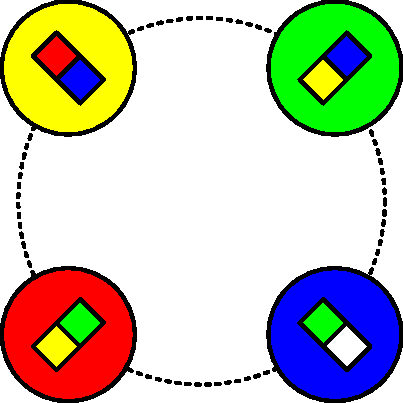
\includegraphics[width=\linewidth]{img/baseball_init.pdf}\\
    \center{État initial}
    \end{column}
    \begin{column}{0.27\linewidth}
    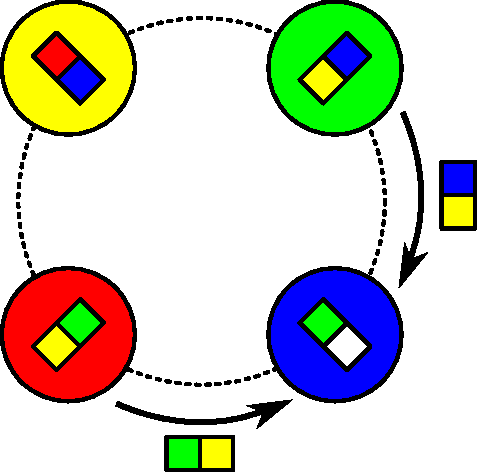
\includegraphics[width=\linewidth]{img/baseball_coup.pdf}\\
    \center{Coup autorisé}
    \end{column}
    \begin{column}{0.27\linewidth}
    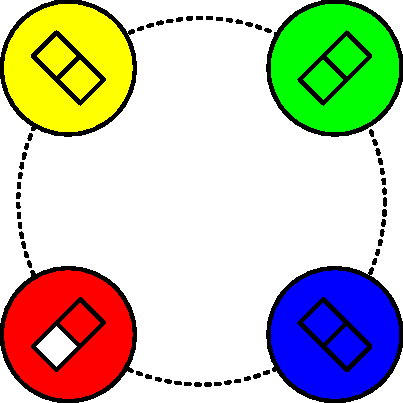
\includegraphics[width=\linewidth]{img/baseball_final.pdf}\\
    \center{État final}
    \end{column}
  \end{columns}

  \bigskip
  \begin{block}{Objectif de l'activité}
    Le plus important dans cet exercice n'est pas tant de résoudre le problème que d'\structure{expliquer clairement} comment on fait. On cherche donc l'\alert{algorithme} permettant de résoudre le problème.
  \end{block}
\end{frame}
%%%%%%%%%%%%%%%%%%%%%%%%%%%%%%%%%%%%%%%%%%%%%%%%%%%%%%%%%%%%%%%%%%%%%%%%%%%%%%%%%%%%%%%%%
%\newcommand{\flecherond}[1]{
  %\draw[ultra thick] (0,0) circle (3mm);
  %\draw[ultra thick,rotate=#1*72] (3mm,0) -- +(-.15,-.08);
  %\draw[ultra thick,rotate=#1*72] (3mm,0) -- +(.08,-.15);
  %\draw[fill=white,draw=white,rotate=#1*72] (3mm,2.5pt) circle (2pt);
%}
\begin{frame}{Un premier algorithme pour le base-ball multicolore}
  En suivant les règles du jeu, on observe que quelque soit la disposition des bonshommes, il existe toujours 4 coups possibles : déplacer vers la case vide un des 4 bonshommes présents dans les deux maisons voisines.

  Notre algorithme sera donc une méthode permettant de choisir à chaque étape quel coup jouer parmis les 4 possibles.

  \begin{block}{L'algorithme}
    \begin{itemize}
    \item On ne s'autorise à tourner que dans un seul sens. Ainsi, le nombre de coups possibles descends de 4 à 2 (car 2 bonshommes tourneraient à l'envers).
    \item Parmis les 2 coups restants, on déplace le bonhomme qui a la plus grande distance à parcourir avant d'arriver à sa maison (Si la distance est la même, c'est que les deux bonhommes ont la même couleur - les deux coups sont donc équivalents).
    \end{itemize}
  \end{block}

  \begin{block}{Exemple d'exécution}
    \begin{center}
      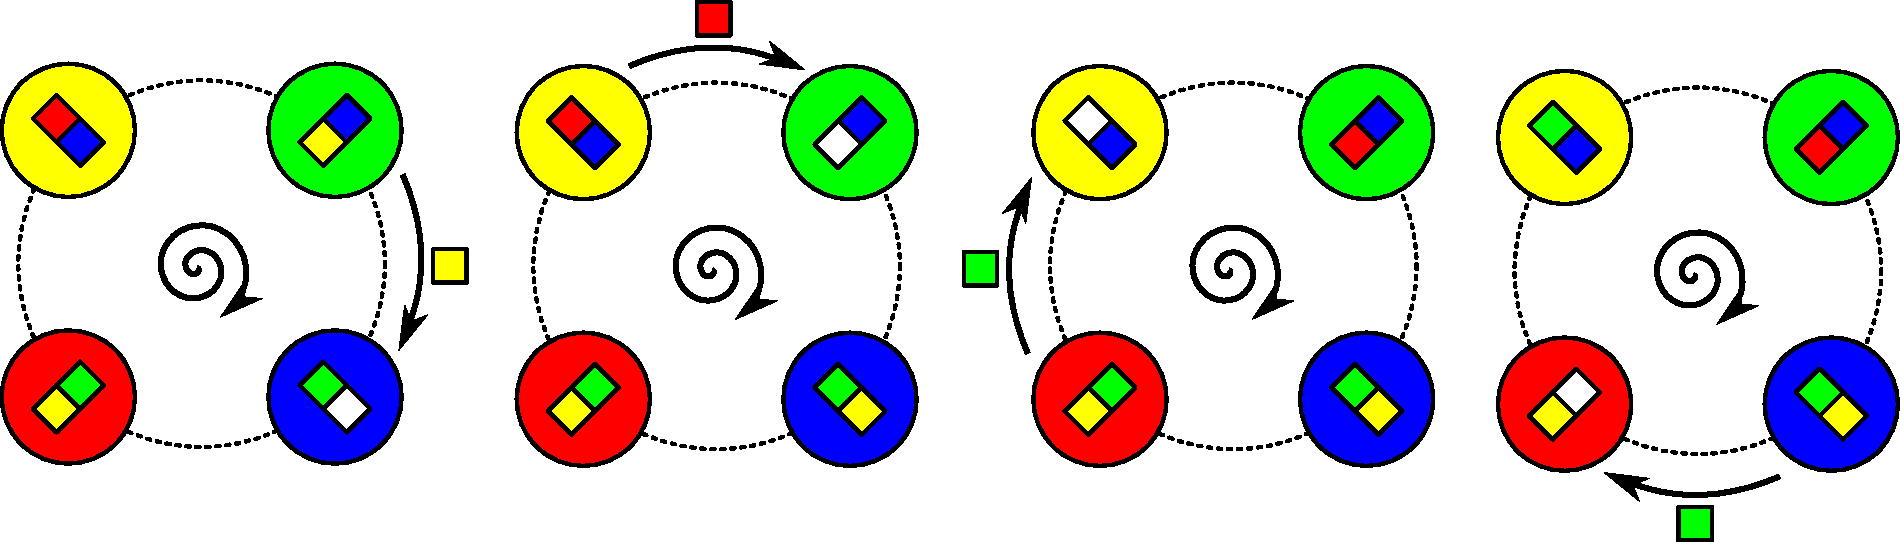
\includegraphics[width=\linewidth]{img/baseball_ex1.pdf}
    \end{center}

  Ici, nous n'avons représenté que les 4 premières étapes. mais l'algorithme arrive à la solution en 15 étapes.
  \end{block}
\end{frame}

\begin{frame}{Étude du premier algorithme pour le base-ball multicolore}
  \begin{block}{Cet algorithme semble attirant}
    \begin{itemize}
    \item Il est très simple: on pourrait l'expliquer à un ordinateur
    \item Il est relativement rapide: 15 coups pour 7 bonshommes, ce n'est pas si mal
    \item Seul problème: cet algorithme est faux: dans certains cas, il ne termine jamais\ldots
    \end{itemize}
  \end{block}

  \begin{block}{Exemple d'exécution incorrecte}
    Il suffit de partir d'une situation gagnée et d'inverser deux bonshommes pour mettre notre algorithme en échec.
\end{block}
  \begin{center}
    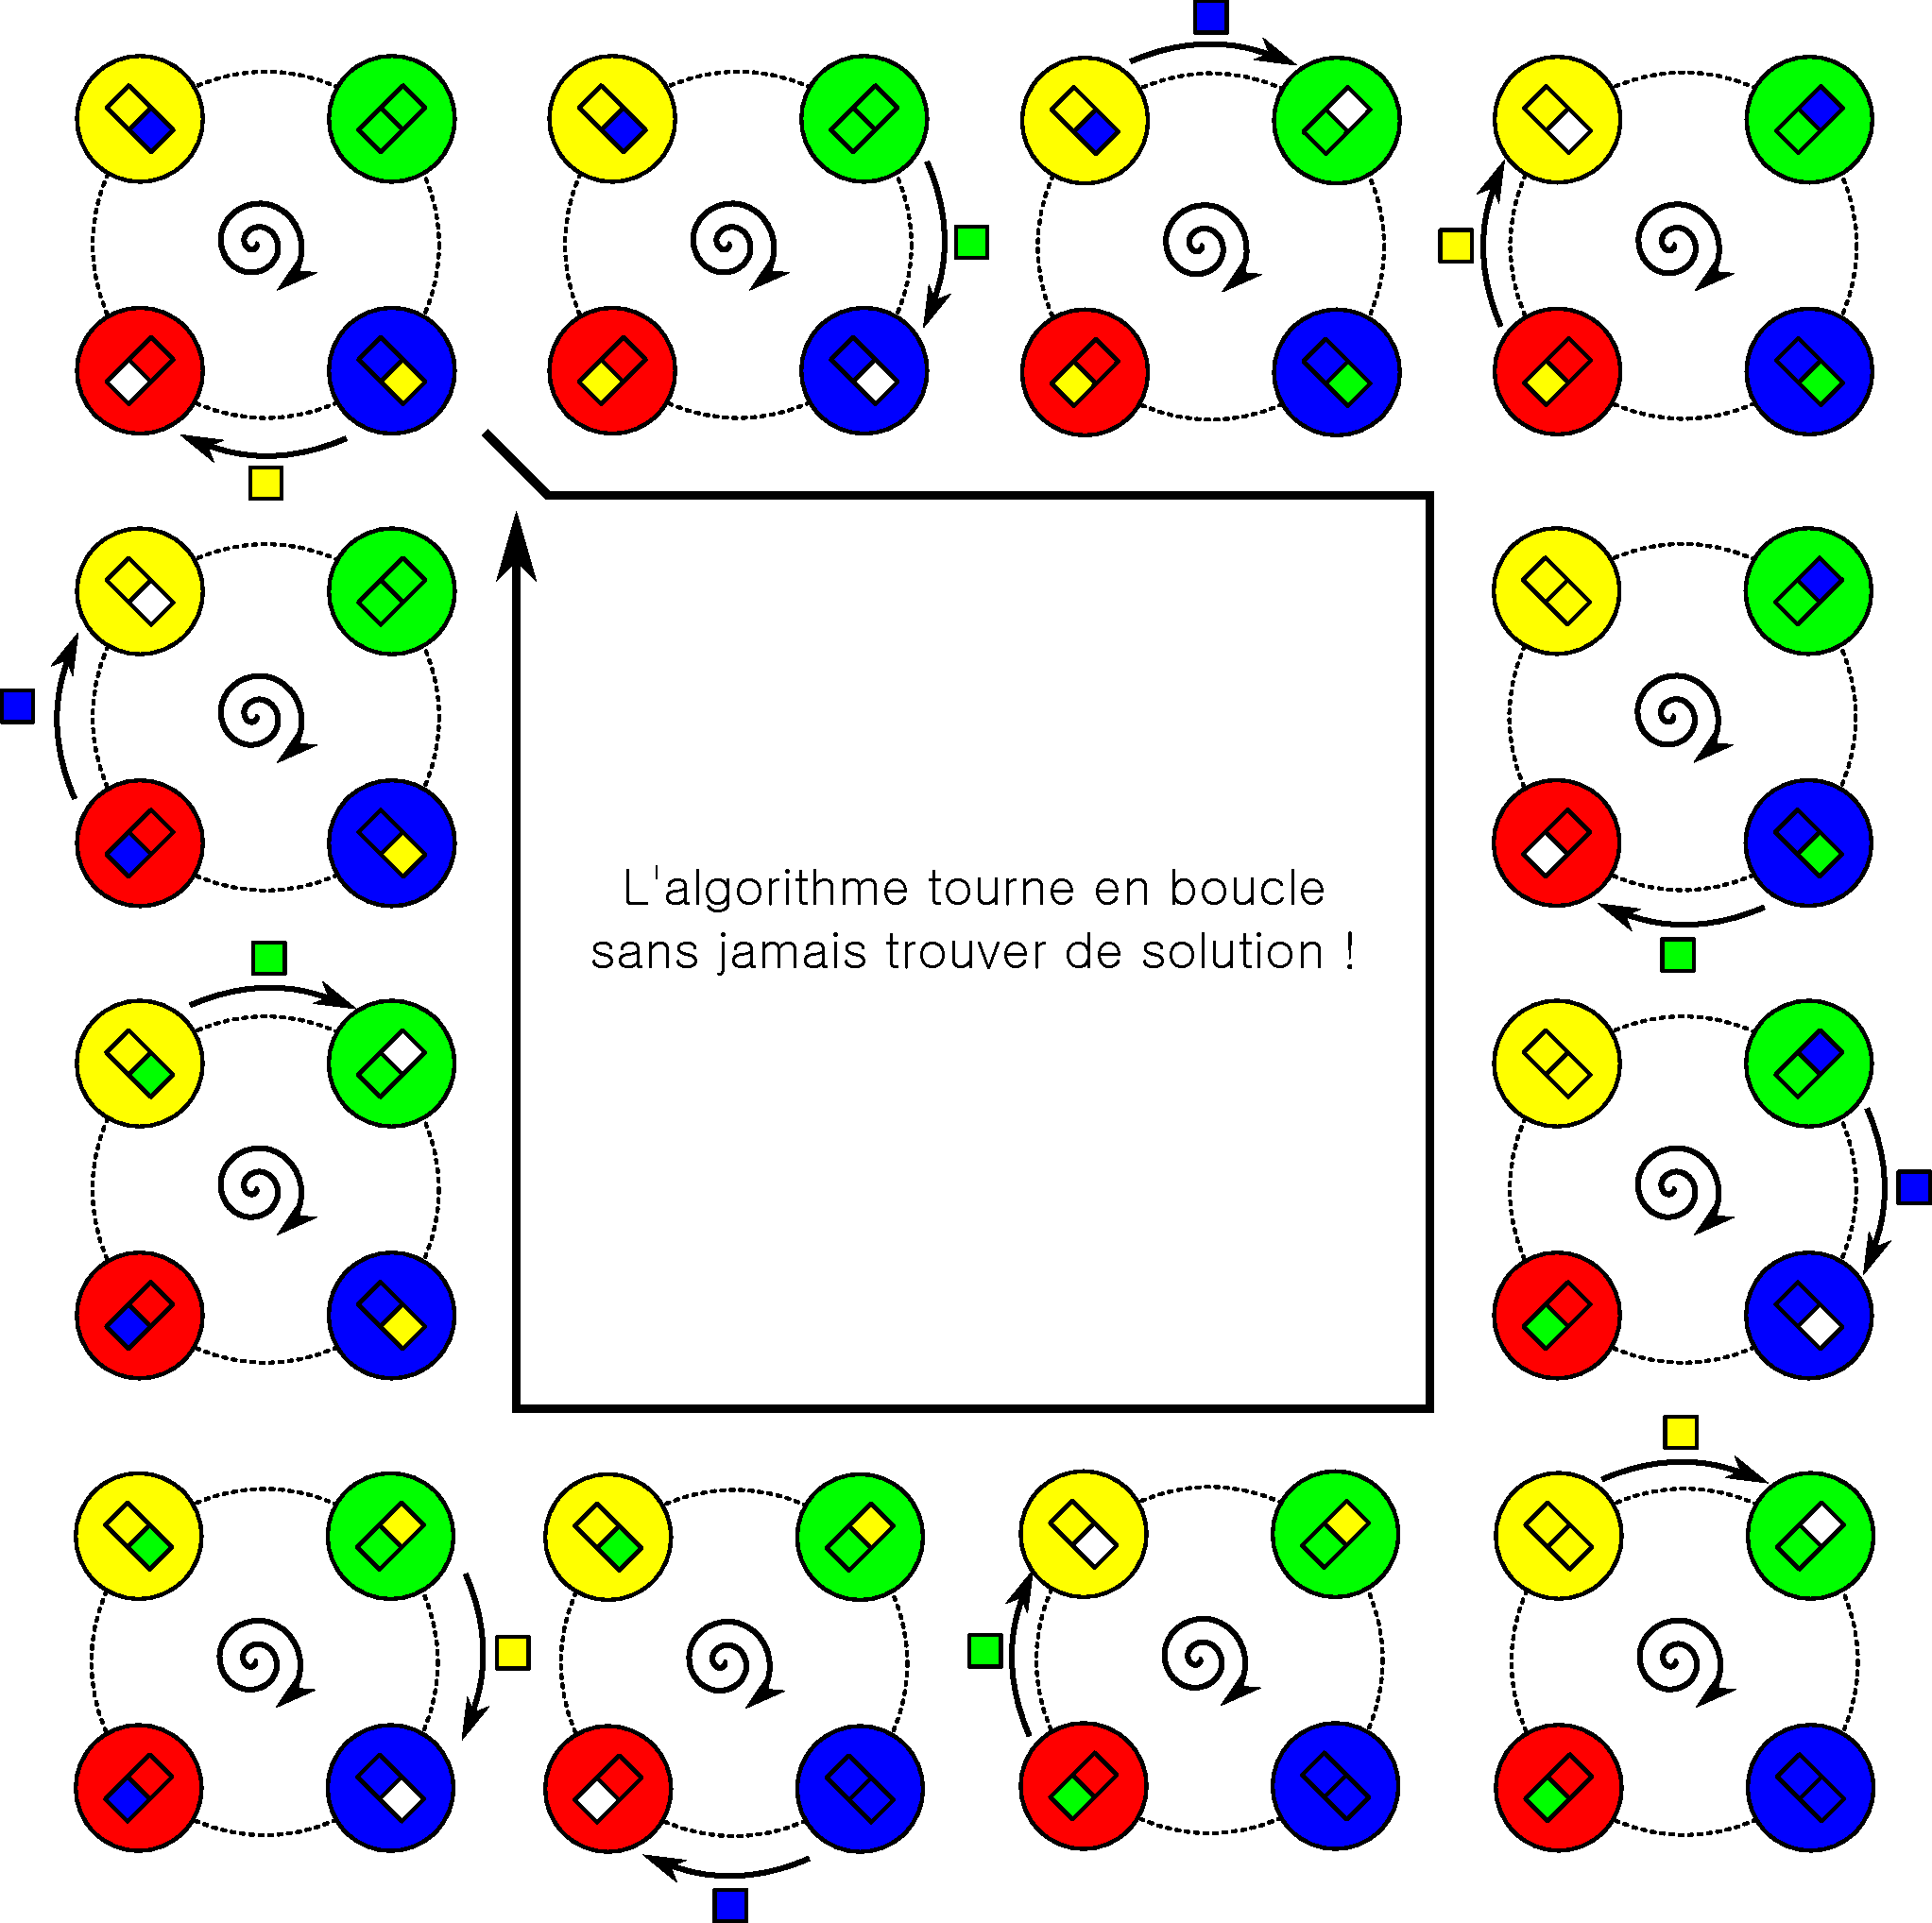
\includegraphics[width=0.8\linewidth]{img/baseball_ex2.pdf}
  \end{center}
\end{frame}

%%%%%%%%%%%%%%%%%%%%%%%%%%%%%%%%%%%%%%%%%%%%%%%%%%%%%%%%%%%%%%%%%%%%%%%%%%%%%%%%%%%%%%%%
\begin{frame}{Un autre algorithme pour le base-ball multicolore}
  \begin{block}{Apprendre de ses échecs: {\color{black}notre algorithme boucle parfois à l'infini}}
    \begin{itemize}
    \item Pour réparer cela, le plus simple est de s'interdire de boucler, en
      coupant le cercle.
    \item Pour ne pas se tromper, le plus simple est de placer les maisons en ligne.
    \end{itemize}

    \begin{center}
      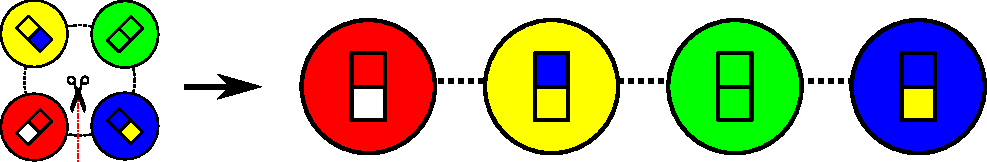
\includegraphics[width=0.8\linewidth]{img/baseball_ligne.pdf}
    \end{center}
  \end{block}

  \bigskip

  \begin{block}{Apprendre de ses réussites: {\color{black}le crépier}}
    \begin{itemize}
    \item On a cherché à réduire la taille du problème à peu à peu\\
      {(il y a 7 crèpes à trier. La plus grande va définitivement à sa place; il
        reste 6 crèpes à trier)}
    \item On s'est fixé des objectifs intermédiaires, qui décomposent le
      problème en étapes que je sais faire\\
      {(mettre la plus grande en haut pour parvenir à la mettre en bas)}
    \end{itemize}
  \end{block}

  \begin{block}{Nouvel algorithme}
    \begin{itemize}
    \item On s'occupe d'abord des bonshommes de la première maison, et on n'y touche plus ensuite.
    \item On répète pour la deuxième maison, et ainsi de suite pour toutes les autres.
    \item Pour ammener les bonhommes dans leur maison, on déplace tous ceux qui gènent.
    \item Pour déplacer ceux qui gènent, on déplace le trou pour leur faire de la place.
    \end{itemize}
  \end{block}

  \begin{center}
    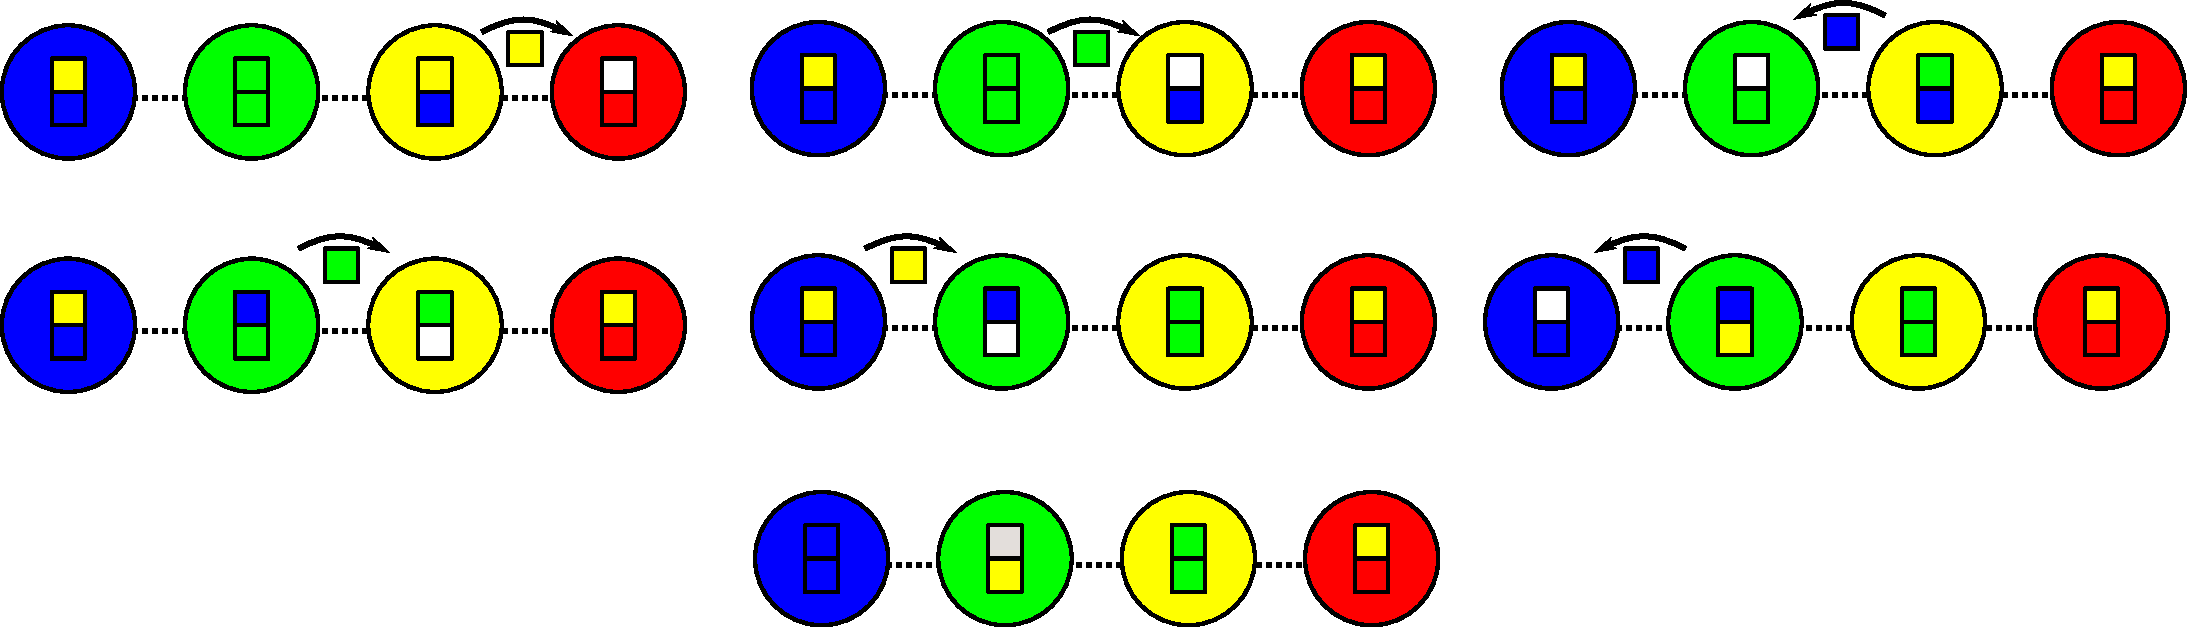
\includegraphics[width=0.8\linewidth]{img/baseball_ex3.pdf}
  \end{center}

  \begin{itemize}
  \item On peut maintenant oublier les bonshommes de la première maison, qui sont à leur place définitive.
  \item On recommence de la même manière avec la deuxième maison, et ainsi de suite ...
  \end{itemize}
\end{frame}

\begin{frame}{Ce qu'il faut retenir du base-ball multicolore: corrections d'algorithmes}
  Cet algorithme n'est pas tellement plus complexe ou plus long que le
  précédent, mais il est correct, lui.

  \begin{block}{Comment être sûr de la \alert{correction} de cet algorithme?}
    \begin{itemize}
    \item \structure{On pourrait tester tous les cas}. Ici, il n'y a pas de limite au nombre de maisons - il est donc impossible de vérifier tous les cas, tout comme il est impossible de compter jusqu'à l'infini. Cependant, on peut se contenter d'une preuve partielle en se limitant à tester tous les cas succeptibles d'être rencontrés - par exemple jusqu'à 20 ou 50 maisons.
    \item \structure{On pourrait écrire une preuve mathématique}. Ce n'est pas trivial, mais les chercheurs en informatique en ont écrite des plus difficiles.
    \item \structure{Cela ressemble vraiment à un algorithme classique} (même
      si cela ne prouve rien, au fond).
    \end{itemize}
  \end{block}

  \begin{block}{Qu'est ce qu'un \alert{algorithme classique}?}
    \begin{itemize}
    \item Les informaticiens apprennent par cœur des algorithmes (abstraits) à l'école.
    \item Face à un problème nouveau, on cherche à se raccrocher à des problèmes connus.
      \begin{itemize}
      \item On se raccroche en trouvant des analogies ou en décomposant en plusieurs problèmes connus.
      \item Par exemple, quand des collègues informaticiens jouent au crêpier, ils demandent avant tout si c'est "une tour de Hanoï".
      \end{itemize}
    \item Ici, notre algorithme est proche d'un "tri à bulle", autre algorithme bien connu. Mais cette ressemblance ne suffit pas à prouver la correction de notre algorithme. Pour la prouver, on pourrait démontrer que notre algorithme est un cas particulier du tri à bulle.
    \end{itemize}
  \end{block}

  \begin{block}{Les algorithmes de tri sont ultra classiques en informatique}
    \begin{itemize}
    \item Ils sont assez simple pour expliquer les grandes lignes aux élèves\\
      (comme «diviser pour régner» et autres grandes idées similaires -- récursivité, algorithmes gloutons, \ldots)
    \item Les ordinateurs trient très souvent des données, car beaucoup de problèmes sont plus simples après\\
      (trouver un livre donné est plus simple dans une bibliothèque rangée, par exemple)
    %\item Du coup, au chapitre 2 de mon cours d'algorithmique, on apprend 5
      %algorithmes de tri par cœur: Tri à bulle, tri par sélection, tri par
      %insertion, tri fusion, tri rapide (et quinze autres en exos).
    \item \alert{Les musiciens font leurs gammes, les informaticiens débutants
      apprennent leurs algorithmes}
    \end{itemize}
  \end{block}

  \begin{block}{Que font les chercheurs en informatique?}
    \begin{itemize}
    \item Certains d'entre eux améliorent les algorithmes connus, ou en
      inventent de nouveaux
    \item Il faut également démontrer la correction de ces algorithmes
    \item Quand plusieurs algorithmes existent, on étudie leurs \alert{performances} respectives
    \item (d'autres chercheurs améliorent matériel et logiciel, établissent des
      modèles, etc)
    \end{itemize}
  \end{block}
\end{frame}

\begin{frame}{Ce qu'il faut retenir du base-ball multicolore: performance d'algorithmes}
  \begin{block}{Comment comparer la performance des algorithmes?}
    \begin{itemize}
    \item Simplement en comptant les étapes. Par exemple sur le crépier, placer la grande crêpe prend au pire 3 coups - et c'est pareil pour les crêpes suivantes. Donc, dans le pire des cas notre algorithme prendra $3\times n$ coups pour trier la pile.
    \item La performance de mon algo dépend beaucoup de la situation initiale:
      \begin{itemize}
      \item Si c'est déjà trié, c'est de la chance, je n'ai rien à faire
        (\alert{meilleur cas}).
      \item Si j'ai vraiment pas de bol, je dois faire les 3 étapes pour chaque crêpe (\alert{pire cas}).
      \item En pratique, j'ai souvent une situation initiale intermédiaire (\alert{cas moyen}).
      \end{itemize}

      Il faut bien comprendre que ceci ne dépend pas vraiment de l'algorithme, mais plutôt de la situation initiale. Le pire cas n'est pas un bug de l'algorithme, mais une situation initiale qui n'aide pas vraiment notre façon de faire (pour estimer la performance d'un cas moyen, il faut utiliser des probabilités).
    \item En pratique, une estimation de la performance est suffisante. Savoir
      qu'un algorithme nécessite environ $n^2$ étapes suffit, inutile de préciser que c'est $n^2+4$ ou $n^2-2$, ou même $5\times n^2$ - pour des grandes valeurs de $n$ c'est sensiblement la même chose\ldots On note cette estimation de la complexité $O(n^2)$.
    \end{itemize}
  \end{block}

  \begin{block}{À la recherche du meilleur algorithme possible}
    \begin{itemize}
    \item On arrive parfois à montrer qu'on a le meilleur algorithme possible. Par exemple on ne peut pas trier les éléments en moins de $n$ étapes, car on doit forcément tous les considérer.
    \item On peut aussi prouver qu'un tri comparatif ne peut pas se faire en moins de $n\times log(n)$ étapes, car il n'accumule pas assez d'information pour choisir la bonne permutation en moins d'étapes.
    \item Mais la plupart du temps, on ne sait pas prouver que l'algorithme connu est le meilleur possible. C'est alors le meilleur \textit{connu}, sans être forcément le meilleur \textit{possible}.
    \end{itemize}
  \end{block}

  \begin{block}{À la recherche de problèmes difficiles}
    \begin{itemize}
    \item On peut classifier les problèmes en fonction de la performance des algorithmes les résolvant. \\
      (cela permet de se forger un sens commun de ce qui est faisable avec un ordinateur et éviter les problèmes si difficiles qu'ils sont quasi impossibles)
    \item Il existe énormément de problèmes relativement simples pour lesquels personne ne connaît de bon algorithme, sans que personne n'arrive non plus à démontrer qu'un tel algorithme n'existe pas.
    \item L'activité suivante sera l'occasion d'explorer un peu cette classification des problèmes très durs.
    \end{itemize}
  \end{block}
\end{frame}

%%% Local Variables: 
%%% mode: latex
%%% TeX-master: "CSIRL"
%%% End: 


\hyphenation{meil-leures}

% récupérer un peu de place au dessus des titres
\renewcommand{\chapterheadstartvskip}{\vspace *{-\baselineskip }} 

\newenvironment{encart}[2]
{
  \begin{center}
  \vbox{
  \colorbox{light-blue}{
  \begin{minipage}{\linewidth}
  \begin{center}\textbf{#1}\end{center}
  \end{minipage}}\\
  \colorbox{light-gray}{
  \begin{minipage}{\linewidth}
  #2
  \end{minipage}}
  }
  \end{center}
}

%\titlehead{Computer Science IRL}
\title{Les Algorithmes \\ 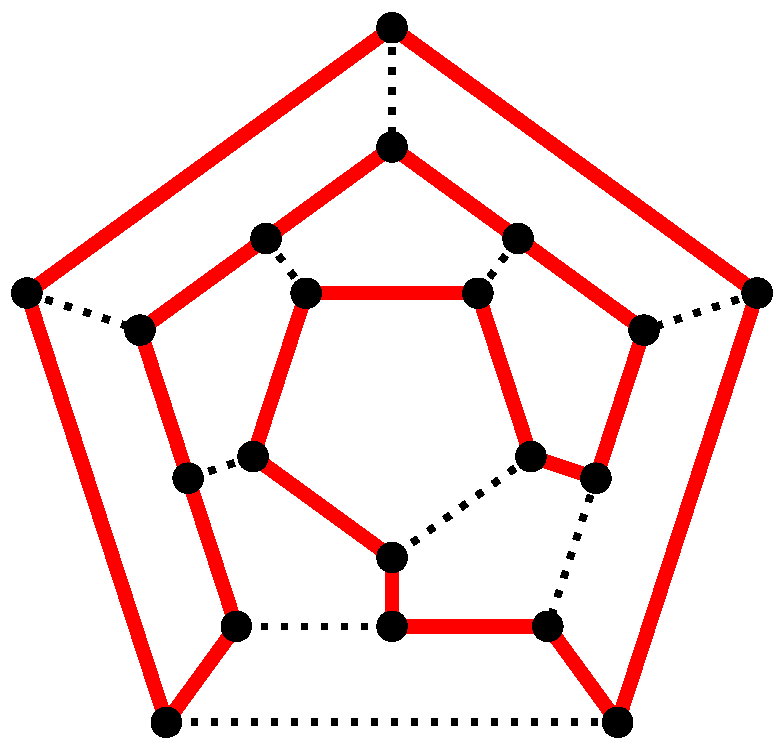
\includegraphics[width=0.7\linewidth]{img/Hamiltonian_path.pdf} \label{img:hamiltonian}}
%\subject{Computer Science IRL}
%\publishers{
\includegraphics[width=5em]{img/pseudo_logo_CSIRL.pdf}} 
\publishers{CS IRL \\ Computer Science In Real Life}
\date{}
%\author{author}

\uppertitleback{
  \copyright\ 2011-2012 membres du projet CS IRL. Tous droits réservés.
  
  CS IRL est un \textbf{projet libre et ouvert}: vous pouvez copier et modifier librement les ressources de ce projet sous les conditions données par la CC-BY-SA (en bref, vous pouvez diffuser et modifier ces ressources à condition que vous donniez les mêmes droits aux utilisateurs de vos copies).
  
  Page web : \url{http://www.loria.fr/~quinson/Mediation/CSIRL/}

  Sources et ressources : \url{http://github.com/jcb/CSIRL}

  Pour nous joindre : \url{discussions@listes.nybi.cc} \\
}

\lowertitleback{
  \textbf{Crédits image}

  \footnotesize

  P\pageref{img:hamiltonian}: Chemin hamiltonien par Ch. Sommer (licence GFDL/CC-BY-SA)\\
  \url{http://en.wikipedia.org/wiki/File:Hamiltonian_path.svg}

  P\pageref{img:CSmajor}: Computer Science Major (licence CC-BY-NC)\\
  \url{http://abstrusegoose.com/206}

%    P\pageref{img:realprog}: Real programmers: \alert{Dessin non libre, à refaire.}
%    \url{http://www.ninisworld.com/oddsends/justforfun/50realprogrammers.html}

  P\pageref{img:tsp}: exemple de TSP adapté de Wikipedia (licence GFDL/CC-BY-SA)\\
  \url{http://en.wikipedia.org/wiki/File:Aco_TSP.svg}
  
  P\pageref{img:tsp_xkcd}: Travelling Salesman Problem par XKCD (licence CC BY-NC 2.5)\\
  \url{http://xkcd.com/399/}
}

\AtBeginDocument{
  \def\labelitemi{$\bullet$}
  \def\labelitemii{$\bullet$}
  \def\labelitemiii{$\bullet$}
}

%\boldmath

\definecolor{light-gray}{gray}{0.95}
\definecolor{light-blue}{rgb}{0.7 0.7 0.9}

\begin{document}

\maketitle

\chapter*{Computer Science IRL\footnote{\textit{Computer Science} signifie science informatique en anglais, tandis que \textit{IRL} est l'abréviation utilisée sur internet pour décrire la vraie vie, ce qui n'est pas sur internet.} -- Informatique sans ordinateur}

%Contrairement à ce que beaucoup de monde pense, les ordinateurs ne sont pas la seule raison d'être de l'informatique. Pour preuve, ce projet développe diverses activités à faire avec des pions, des jetons ou des bouts de bois, mais sans aucun ordinateur et même sans électricité. Pourtant, ces petits jeux permettront à chacun de découvrir de manière ludique les notions au cœur de l'informatique: ce qu'est un algorithme et qu'est ce qui fait qu'un algorithme est meilleur qu'un autre, ou encore comment coder et transmettre une information.

Trop souvent, lorsque l'on parle d'informatique, on pense à l'ordinateur utilisé comme outil. L'informatique devient alors l'art d'utiliser l'ordinateur pour une tâche donnée, ou de le réparer. Pourtant, dans les entrailles de cette machine se cache un domaine scientifique très vaste, dont les ramifications dépassent largement l'ordinateur et son fonctionnement.

Avec le projet \textbf{CS IRL}, nous vous proposons d'explorer la science informatique ... en retirant l'ordinateur ! Pour cela, nous avons conçu une série d'activités ludiques introduisant des notions fondamentales de l'informatique par le biais d'un support matériel, pour \textit{apprendre avec les mains}. Ces activités sont regroupées en séances thématiques, permettant ainsi d'aborder les notions fondamentales de manière cohérente et progressive.

%\begin{block}{Introduction: les principales caractéristiques d'un ordinateur}
    %\begin{itemize}
    %\item \structure{Il est très \alert{rapide}:} il peut calculer de 1 à 1
      %million en moins d'une seconde
    %\item \structure{Il est parfaitement \alert{obéissant}:} il fait
    %tout le temps exactement ce qu'on lui demande
    %\item \structure{Il est absolument \alert{stupide}:} il exécute les
      %ordres qu'on lui donne, sans la moindre capacité d'initiative.
      %\begin{itemize}
      %\item Par exemple, si on demande à un ordinateur de s'arrêter, il le fait\ldots
      %\item Autre exemple, quand j'indique à des amis comment venir chez moi,
        %je leur donne des indications comme ``troisième à droite'' ou ``à gauche
        %au 2ieme feu''. Si je me trompe dans mes indications (``à gauche'' au lieu
        %de ``à droite'') et que cela les ferait prendre l'autoroute à
        %contre-sens, mes amis vont faire preuve de sens commun et ne pas
        %appliquer la consigne. Les ordinateurs n'ont \textbf{aucun} sens commun.
      %\item Bug (n.m.): consigne erronée donnée par un humain et appliquée bêtement par une machine.
      %\end{itemize}
    %\end{itemize}
  %\end{block}\vspace{-.5\baselineskip}

\section*{La séance algorithmique}

L'objectif de cette séance est d'introduire la notion fondamentale d'\textbf{al\-gorithme}. Qu'est ce que c'est ? A quoi ça sert ? Comment sont ils inventés ? Pour cette séance, comptez \textbf{une heure et demie à deux heures}. Si vous êtes animateur, vous trouverez des conseils et des astuces dans le coin de l'animateur en page \pageref{chap:coin-animateur}.

Bien entendu, il ne s'agit pas d'un cours complet sur le sujet ! Si vous souhaitez aller plus loin, voici un cours en 48h : \url{http://www.loria.fr/~quinson/Teaching/TOP/}.

\begin{center}
  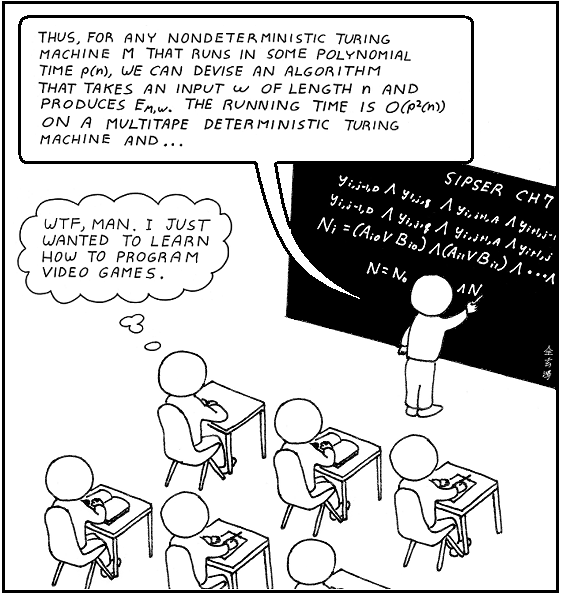
\includegraphics[width=0.7\linewidth]{img/computer_science_major.PNG}
  \label{img:CSmajor}
\end{center}

\chapter*{Le jeu de Nim}

Voici un premier petit jeu simple, pour rentrer dans le sujet. On dispose sur une table \textit{16 objets}. Chacun leur tour, les deux joueurs ramassent \textit{un, deux ou trois objets} sur la table. Le joueur qui \textbf{ramasse le dernier objet} remporte la partie.

\bigskip
 
\encart{Matériel}{
  \begin{itemize}
    \item 16 petits objets (clous, allumettes ... peu importe !)
  \end{itemize}
}

\bigskip
\bigskip
\bigskip

%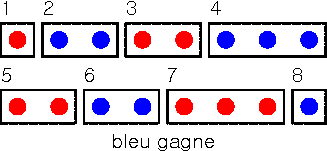
\includegraphics[width=\linewidth]{img/nim.pdf}
\begin{center}
\newcommand\red[1]{
  \node [circle,fill=red,text=black] {\textbf #1}
}

\newcommand\blue[1]{
  \node [circle,fill=blue,text=white] {\textbf #1};
}

\begin{tikzpicture}

\matrix (m) [nodes={draw, thick}, row sep=0.3cm, column sep=0.3cm] {
  \red{1}; &
  \blue{2}; &
  \blue{2}; &
  \red{3}; &
  \red{3}; &
  \blue{4}; &
  \blue{4}; &
  \blue{4}; \\
  \red{5}; &
  \red{5}; &
  \blue{6}; &
  \blue{6}; &
  \red{7}; &
  \red{7}; &
  \red{7}; &
  \blue{8}; \\
};

\end{tikzpicture}
 \\
\textbf{Le joueur bleu gagne}
\end{center}

\newpage

\section*{Stratégie gagnante}

Le jeu de Nim est sans suspense : le premier à jouer perd, car il existe une astuce pour que le deuxième joueur gagne à tous les coups. La \textbf{stratégie gagnante} est de laisser 4, 8, 12 ou 16 objets à l'adversaire (un multiple de 4).

Pour se convaincre de l'efficacité de la stratégie gagnante, prenons le dernier tour comme exemple. Il reste 4 objets, et J1 joue :

\begin{itemize}
  \item si J1 prend 1 objet, J2 en prend 3 (dont le dernier) ;
  \item si J1 prend 2 objets, J2 en prend 2 (dont le dernier) ;
  \item si J1 prend 3 objets, J2 en prend 1 (le dernier).
\end{itemize}        

Dans ce cas, si J2 sait jouer, J1 perd à tous les coups. En appliquant la même méthode, J2 peut guider le jeu de manière à passer de 16 objets à 12, puis 8 et enfin 4. Donc, si J2 sait jouer, J1 a perdu la partie avant même de commencer.

\begin{center}
  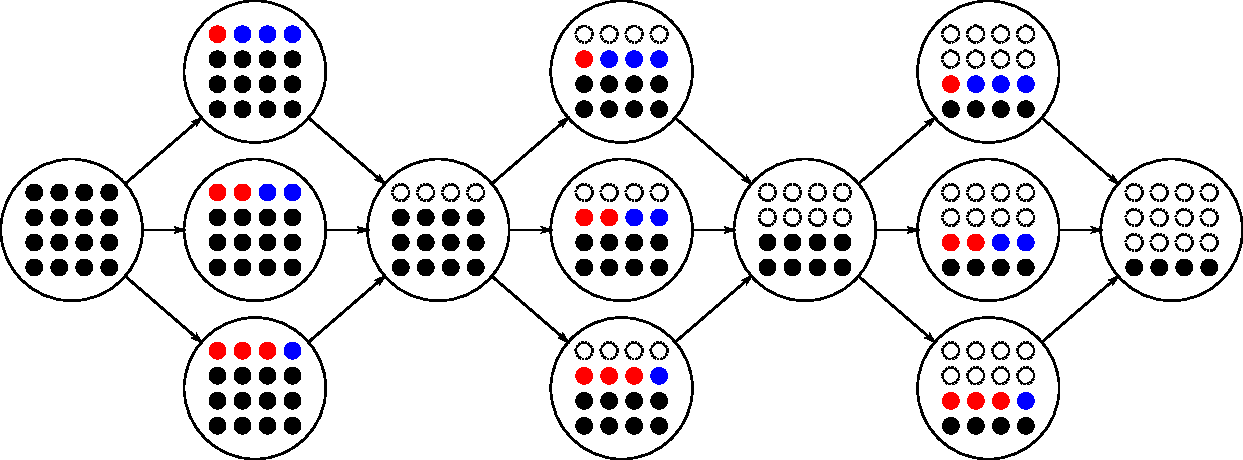
\includegraphics[width=\linewidth]{img/nim16.pdf}
\end{center}

\subsection*{Rapport avec l'informatique}

Comme pour le jeu de Nim, \textbf{un algorithme est une stratégie gagnante} permettant de trouver la solution à un problème donné. Dans l'exemple précédent, le problème était «comment gagner au jeu de Nim ?»

\encart{Pour aller plus loin}{
  On pourrait imaginer un cas plus général du jeu de Nim :

  \begin{itemize}
    \item Il y a $N$ objets sur la table au début du jeu \\ (pour notre version, $N=16$)
    \item Un joueur peut prendre jusqu'à $X$ objets à la fois \\ (pour notre version, $X=3$)
  \end{itemize}

  Quelles modifications doit-on apporter à notre stratégie gagnante pour qu'elle marche dans le cas général ?
}

\chapter*{Le crêpier psycho-rigide}

A la fin de sa journée, un crêpier dispose d'une pile de crêpes désordonnée. Le crêpier étant un peu psycho-rigide, il décide de ranger sa pile de crêpes, de la plus grande (en bas) à la plus petite (en haut), avec le coté brûlé caché. 

\begin{center}
  \begin{frame}{Activité: Le crêpier psycho-rigide}

  \begin{block}{Matériel}
    \begin{itemize}
    \item des planchettes en bois de tailles et de couleurs différentes (faces reconnaissables)
    \item éventuellement une pelle à tarte pour retourner les planchettes
    \end{itemize}
  \end{block}

  \begin{block}{Règle du jeu}
    \begin{itemize}
      \item \structure{Installation :} Faire une pile désordonnée de crêpes.
      \item \structure{Objectif :} ranger les crêpes de la plus grande (en bas) à la plus petite (au haut), face colorée vers le haut.
      \item \structure{Coup autorisé :} prendre une ou plusieurs crêpes sur le haut de la pile, et de les reposer à l'envers.
    \end{itemize}
  \end{block}

  \bigskip \bigskip \bigskip

  \begin{center}
    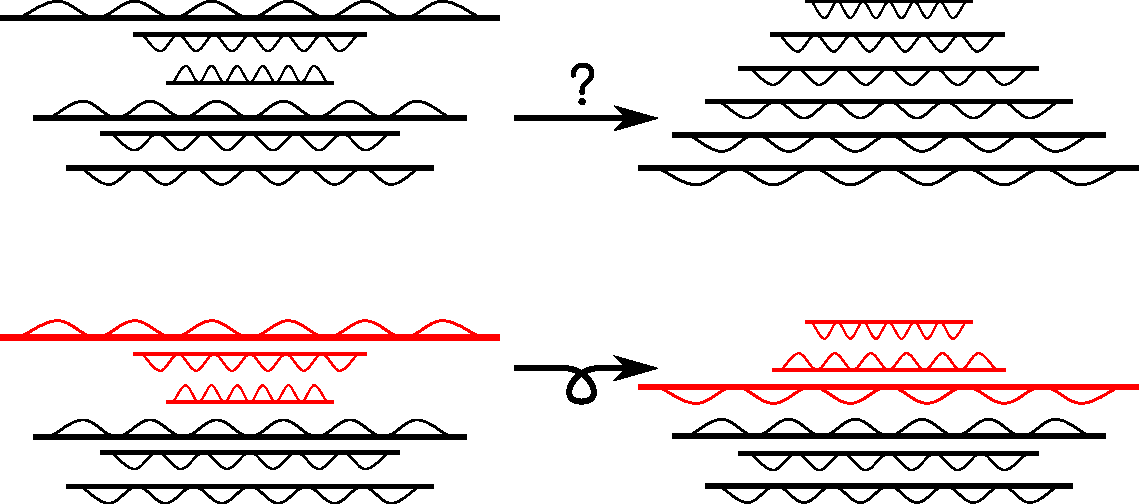
\includegraphics[width=0.8\linewidth]{img/crepier.pdf}
  \end{center}

\end{frame}

\begin{frame}{Ce qu'il faut retenir du  crêpier psycho-rigide}

  \begin{columns}
    \begin{column}{.7\linewidth}
      \begin{block}{Un algorithme}
        \begin{itemize}
        \item n'a d'intérêt que si on peut l'expliquer
        \item doit être suffisamment simple pour pouvoir l'expliquer à une machine
        \item \alert{\textbf{«Diviser pour mieux régner»}} : on essaie toujours de décomposer un algorithme en tâches simples
        \end{itemize}
      \end{block}

      \begin{block}{L'algorithme que doit suivre le crêpier est :}
        \begin{itemize}
        \item ramener la plus grande crêpe en haut de la pile
        \item retourner pour que la face brûlée soit vers le haut
        \item retourner la pile de sorte à mettre la plus grande crêpe en bas
        \item réitérer avec la crêpe de taille inférieure
        \end{itemize}
      \end{block}

      \begin{block}{Le rapport avec l'informatique}
        \begin{itemize}
        \item l'informaticien passe son temps à trouver des algorithmes et  à les expliquer à la machine
        \item le principe \alert{\textbf{«Diviser pour mieux régner»}} est fondamental en informatique
        \end{itemize}
      \end{block}
    \end{column}

    \begin{column}{.3\linewidth}
      \begin{block}{Pour aller plus loin}
        Selon l'état initial de la pile de crêpes, le nombre minimum de coups nécessaires pour la ranger varie.

        \begin{itemize}
          \item Quel est le meilleur état initial possible (qui demandera le moins de coups pour ranger) ?
          \item Quel est le pire état initial possible ?
          \item Combien faut-il de coups pour ranger une pile de $N$ crêpes dans le pire des cas ?
        \end{itemize}
      \end{block}
    \end{column}
  \end{columns}
      
\end{frame}

\begin{frame}{Ce qu'il faut retenir du crêpier psycho-rigide : performance d'algorithmes}

  \begin{block}{Pourquoi évaluer la performance d'un algorithme ?}

    Évaluer la performance d'un algorithme nous permet :

    \begin{itemize}
      \item de se faire une idée du temps nécessaire pour résoudre un problème de plus grande taille (combien de temps pour un million de crêpes ?) ;
      \item de le comparer à d'autres aglorithmes résolvant le même problème, pour savoir lequel est le meilleur.
    \end{itemize}

  \end{block}

  \begin{block}{Comment évaluer la performance d'un algorithme ?}

    \begin{itemize}
      \item On compte le nombre de coups nécessaires dans le cas général. Pour le crêpier :
        \begin{itemize}
          \item pour ranger une crêpe, il faut entre $0$ coups (la crêpe est déjà rangée) et $3$ coups (amener en haut, retourner, amener à sa place) ;
          \item pour $n$ crêpes (cas général), il faut entre $0$ et $3 \times n$ coups ;
          \item la performance d'un algorithme sur un cas particulier dépend donc beaucoup de l'état initial, mais en règle générale on s'intéresse surtout aux cas intermédiaires, qui sont les plus probables.
        \end{itemize}
      \item $n$ est une variable qui exprime la taille du problème. La performance d'un algorithme est notée comme une fonction de la taille du problème nommée $O$.
      \item La performance exprime un ordre de grandeur plutôt qu'une évaluation précise du temps d'exécution. Pour des grandes valeurs de $n$, il n'est pas très utile de faire la distinction entre $O(n)$, $O(n+4)$ ou encore $O(3 \times n)$ - surtout quand on compare avec un autre algorithme dont la performance est $O(n^2)$. 
      \item On simplifie donc en retirant les constantes pour ne garder que les termes les plus importants. Pour le crêpier, on notera la performance de notre algorithme $O(n)$ ; on dit alors que le temps de calcul croit \textit{linéairement} avec $n$. En revanche, un algorithme $O(n^2)$ aurait une croissance \textit{quadratique}, et un algorithme $O(2^n)$ aurait une croissance \textit{exponentielle}.
     \end{itemize}
  \end{block}

  \begin{block}{À la recherche du meilleur algorithme possible}
    \begin{itemize}
    \item On arrive parfois à montrer qu'on a le meilleur algorithme possible. Par exemple on ne peut pas trier les éléments en moins de $n$ étapes, car on doit forcément tous les considérer.
    \item On peut aussi prouver qu'un tri comparatif ne peut pas se faire en moins de $n\times log(n)$ étapes, car il n'accumule pas assez d'information pour choisir la bonne permutation en moins d'étapes.
    \item Mais la plupart du temps, on ne sait pas prouver que l'algorithme connu est le meilleur possible. C'est alors le meilleur \textit{connu}, sans être forcément le meilleur \textit{possible}.
    \end{itemize}
  \end{block}

  %\begin{block}{À la recherche de problèmes difficiles}
    %\begin{itemize}
    %\item On peut classifier les problèmes en fonction de la performance des algorithmes les résolvant. \\
      %(cela permet de se forger un sens commun de ce qui est faisable avec un ordinateur et éviter les problèmes si difficiles qu'ils sont quasi impossibles)
    %\item Il existe énormément de problèmes relativement simples pour lesquels personne ne connaît de bon algorithme, sans que personne n'arrive non plus à démontrer qu'un tel algorithme n'existe pas.
    %\item L'activité suivante sera l'occasion d'explorer un peu cette classification des problèmes très durs.
    %\end{itemize}
  %\end{block}
\end{frame}

\end{center}

Pour cette tâche, le crêpier peut faire une seule action : glisser sa spatule entre deux crêpes et retourner le haut de la pile. Comment doit-il procéder pour trier toute la pile ?

\begin{center}
  \newcommand{\crepe}[5]{ % size yshift xshift flip
	\draw [color=#5, dashed, thick, yshift=#2*0.4cm, xshift=#3cm,rotate=#4*180] (-#1,0.1) -- (#1,0.1);
	\draw [color=#5, thick, yshift=#2*0.4cm, xshift=#3cm,rotate=#4*180](-#1,0.1) -- (-#1,-0.1) -- (#1,-0.1) -- (#1,0.1);
}

\begin{tikzpicture}[scale=0.8]

% \crepe{1cm}{0}{180};
% \crepe{1.5cm}{(0,1.5)}{0};
% \crepe{2cm}{(0,0)}{180};
% \crepe{2.5cm}{(0,1)}{0};
% \crepe{3cm}{(0,2)}{0};

\crepe{3cm}{4}{0}{1}{red};
\crepe{2cm}{3}{0}{0}{red};
\crepe{1.5cm}{2}{0}{0}{red};

% dessin de la pelle à tarte (une pelle à crêpes, ça n'existe pas ?)
\draw [color=black, thick, yshift=2*0.4cm, xshift=0cm,rotate=0*180] (-4,0.2) -- (-2,-0.2) -- (2,-0.2);

\crepe{2.5cm}{1}{0}{0}{black};
\crepe{1cm}{0}{0}{1}{black};

\draw [->,ultra thick,draw] (3,1) -- (5,1) ;

\crepe{1.5cm}{4}{8}{1}{red};
\crepe{2cm}{3}{8}{1}{red};
\crepe{3cm}{2}{8}{0}{red};
\crepe{2.5cm}{1}{8}{0}{black};
\crepe{1cm}{0}{8}{1}{black};


\end{tikzpicture}

\end{center}

\encart{Matériel}{
  \begin{itemize}
  \item des planchettes en bois de tailles et de couleurs différentes (faces reconnaissables)
  \item éventuellement une pelle à tarte pour retourner les planchettes
  \end{itemize}
}

%\begin{center}
  %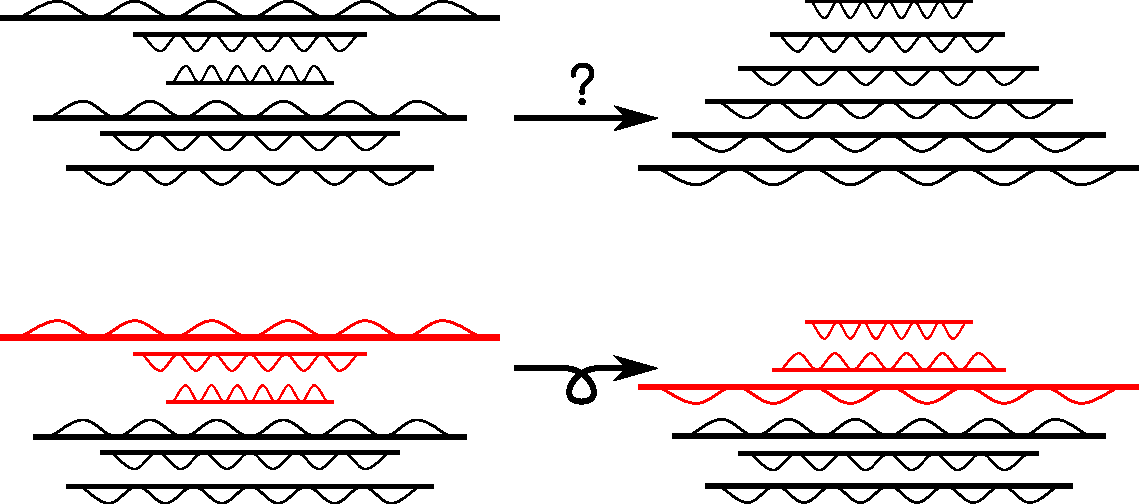
\includegraphics[width=0.6\linewidth]{img/crepier.pdf}
%\end{center}

\newpage

\section*{Description d'un algorithme}

L'algorithme permettant de résoudre le problème du crêpier est le suivant :

\begin{enumerate}
\item amener la plus grande crêpe en haut de la pile
\item mettre la face brûlée vers le haut
\item retourner toute la pile - la crêpe est rangée
\item recommencer en ignorant les crêpes rangées
\end{enumerate}

Cet algorithme assez simple nous apprend deux choses. Premièrement, un algorithme n'a d'intérêt que si on peut l'expliquer - pire encore, que si on peut l'\textit{expliquer à un ordinateur}. Il doit donc être \textbf{écrit sans ambiguîté}. Deuxièmement, un algorithme décompose le problème en une série de tâches simples. On appelle ce principe \textbf{\og Diviser pour mieux régner\fg}.

Ce que nous venons de décrire est le c\oe{}ur de métier des informaticiens : analyser un problème, le subdiviser en problèmes plus simples, formaliser le tout sous la forme d'un algorithme, et traduire l'algorithme dans un langage compréhensible par l'ordinateur.

\section*{Performance d'un algorithme}

Le premier objectif de l'écriture d'un algorithme est qu'il résolve le problème. Le second objectif est qu'il le résolve le plus vite possible. 

Évaluer la \textbf{performance d'un algorithme} nous permet de nous faire une idée du temps nécessaire à la résolution d'un problème de grande taille. Par exemple, combien de temps faudra-t-il à notre algorithme pour trier une pile d'un million de crêpes ?

De plus, s'il existe plusieurs algorithmes résolvant le même problème, l'évaluation de la performance nous donne un critère objectif pour savoir lequel est le plus efficace.

\subsection*{Évaluer la performance d'un algorithme}

Pour évaluer la performance, on compte le nombre de \og coups \fg nécassaires pour résoudre le problème dans le cas général. Pour le problème du crêpier :

\begin{itemize}
  \item pour ranger une crêpe, il faut entre $0$ coup (la crêpe est déjà rangée) et $3$ coups (amener en haut, retourner, amener à sa place) ;
  \item pour $n$ crêpes (cas général), il faut entre $0$ coup (meilleure situation) et $3 \times n$ coups (pire situation). La performance de l'algorithme dépend donc beaucoup de l'état initial, mais on s'intéresse surtout aux cas intermédiaires, qui sont les plus probables.
\end{itemize}

Ici, $n$ est une variable qui exprime la taille du problème. La performance d'un algorithme est notée comme une fonction de la taille du problème nommée $O$. Pour le crêpier, on peut donc écrire $O(3 \times n)$.

Le temps d'exécution variant selon l'état initial, la performance exprime l'ordre de grandeur du temps d'exécution. Pour des grandes valeurs de $n$, il n'est pas très utile de faire la distinction entre $O(n)$, $O(n+4)$ ou encore $O(3 \times n)$ - en particulier quand on compare avec un autre algorithme dont la performance est $O(n^2)$. 

On simplifie donc en retirant les constantes pour ne garder que les termes importants. Pour le crêpier, on notera donc la performance de notre algorithme $O(n)$ ; on dit alors que la performance de l'algorithme est \textit{linéaire}, car le temps de calcul croît linéairement avec $n$. Un algorithme avec une performance $O(n^2)$ est dit \textit{quadratique}, tandis qu'un algorithme $O(2^n)$ est dit \textit{exponentiel}.

\subsection*{À la recherche du meilleur algorithme possible}

On arrive parfois à montrer qu'on a le meilleur algorithme possible. Par exemple, on ne peut pas trier les éléments en moins de $n$ étapes, car on doit forcément tous les considérer.

On peut aussi prouver qu'un tri comparatif ne peut pas se faire en moins de $n\times log(n)$ étapes, car il n'accumule pas assez d'information pour choisir la bonne permutation en moins d'étapes.

Mais la plupart du temps, on ne sait pas prouver que l'algorithme connu est le meilleur possible. C'est alors le meilleur \textit{connu}, sans être forcément le meilleur \textit{possible}.
    
\chapter*{Le Base-ball multicolore}

On dispose de quatre bases de couleurs différentes, et deux joueurs associés à chaque base. Le but du jeu est de déplacer les joueurs afin de ramener chaque joueur sur la base correspondant à sa couleur. Il y a cependant trois contraintes :

\begin{itemize}
  \item les bases sont disposées en cercle, et un joueur ne peut se déplacer que vers les deux bases voisines (il ne peut pas traverser le terrain) ;
  \item on ne peut déplacer qu'un joueur à la fois ;
  \item chaque base a deux places, et un joueur ne peut se déplacer vers une base que si elle possède une place libre.
\end{itemize}

\begin{center}
  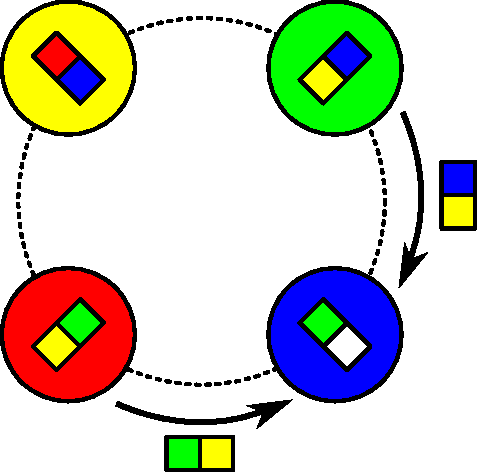
\includegraphics[width=0.3\linewidth]{img/baseball_coup.pdf}
  %\begin{tabular}{cc}
    %\etat{green}{blue}{red}{yellow}{white}{yellow}{green}{blue} &
    %\etat{red}{white}{green}{green}{blue}{blue}{yellow}{yellow} \\
    %État initial &
    %État final \\
  %\end{tabular}
\end{center}

\encart{Matériel}{
  \begin{itemize}
  \item Plusieurs équipes bien différentiables, chacune composée d'une base et de deux joueurs (des legos, des bouts de bois, des cailloux, du fil électrique de différentes couleurs, ou autres) 
  \item 4 équipes au minimum. On peut mettre des équipes ou des joueurs supplémentaires pour augmenter la difficulté.
  \end{itemize}
}

L'objectif de cette activité est d'\textbf{expliquer clairement} la méthode de résolution du problème (algorithme), ainsi que le raisonnement qui a permis de trouver cette méthode.

\newpage

\section*{Premier algorithme}

En suivant les règles du jeu, on observe que quelque soit la disposition des joueurs, 4 joueurs peuvent être déplacés vers la place vide : les deux de la base de gauche, les deux de la base de droite. Notre algorithme sera donc une méthode permettant de choisir à chaque étape quel coup jouer parmi ces 4 possibles.

\begin{itemize}
  \item On ne s'autorise à tourner que dans un seul sens. Ainsi, le nombre de coups possibles descend de 4 à 2 (car 2 joueurs tourneraient à l'envers).
  \item Parmi les 2 coups restants, on déplace le joueur qui a la plus grande distance à parcourir avant d'arriver à sa base (Si la distance est la même, c'est que les deux joueurs ont la même couleur - les deux coups sont alors équivalents).
  \item Tant que tous les joueurs ne sont pas rentrés à leur base, on continue les déplacements.
\end{itemize}

% FIXME tikz ?
\begin{center}
  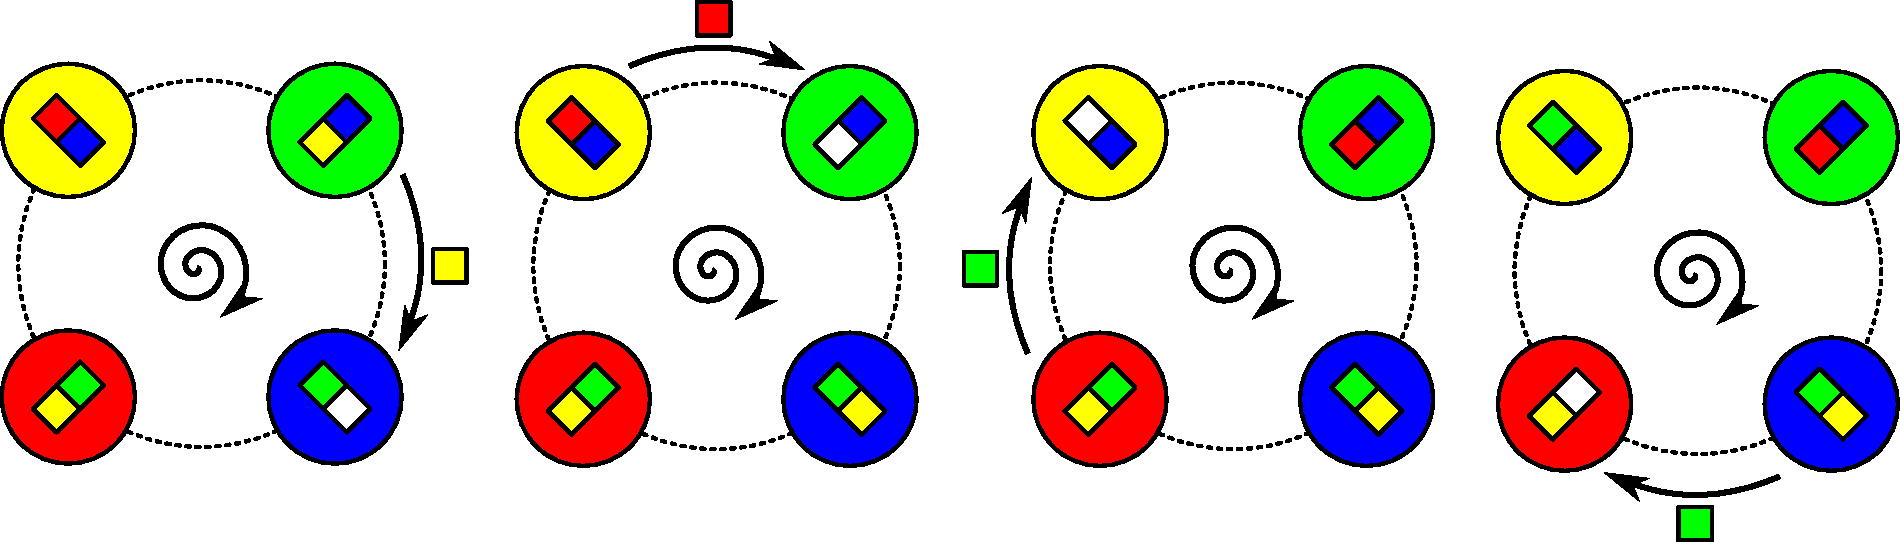
\includegraphics[width=\linewidth]{img/baseball_ex1.pdf}
\end{center}

Ici, nous n'avons représenté que les 4 premières étapes, mais l'algorithme arrive à la solution en 15 étapes.

\subsection*{Regardons plus en détail ...}

À première vue, cet algorithme est attirant : il est assez simple et semble relativement rapide : 15 coups pour 4 bases et 7 joueurs, ce n'est pas si mal. Pourtant, il y a un problème : \textit{cet algorithme est faux}. 

Pour s'en convaincre, il suffit de prendre le jeu dans son état résolu, et d'intervertir deux joueurs. On observe alors que notre algorithme ramène le jeu à son état initial sans atteindre la solution - notre algorithme boucle donc à l'infini.

% FIXME tikz ?
\begin{center}
  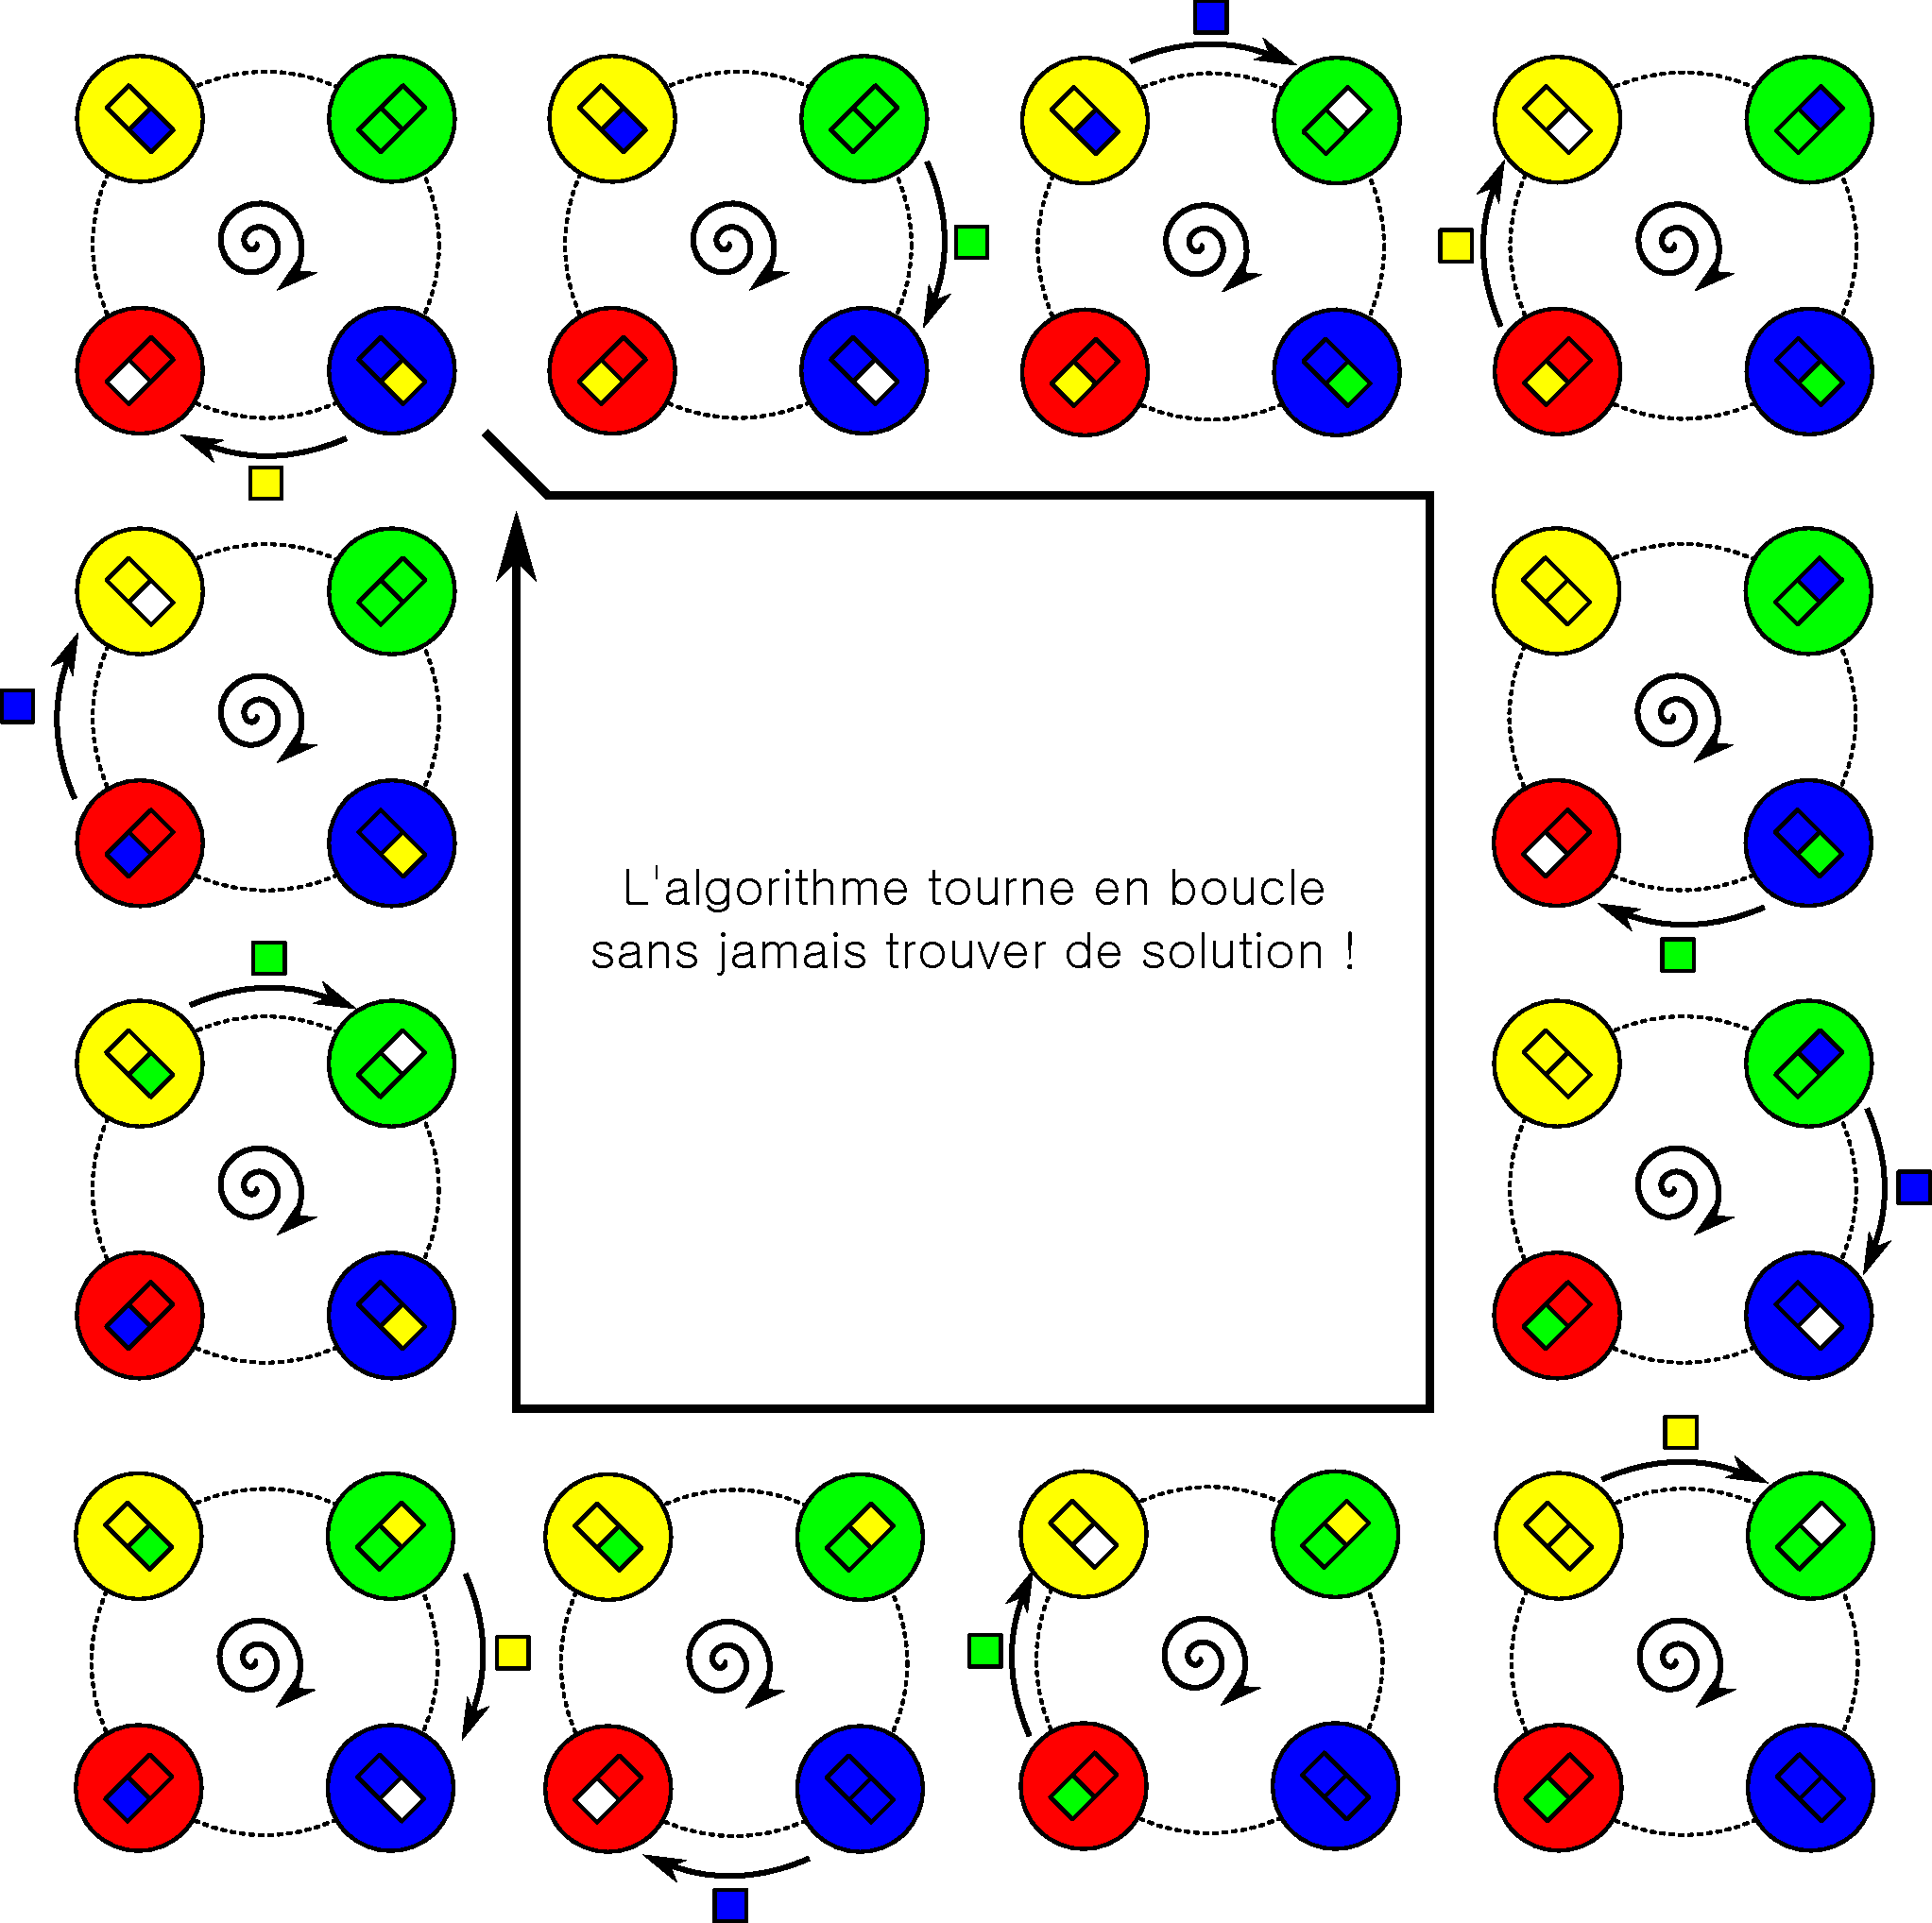
\includegraphics[width=\linewidth]{img/baseball_ex2.pdf}
\end{center}

\newpage

\section*{Deuxième algorithme}

Notre premier algorithme étant faux, réfléchissons à un autre algorithme. 

Commençons par \textit{apprendre de nos échecs}. Notre premier algorithme boucle parfois à l'infini. Pour réparer cela, on pourrait s'interdire de faire un tour complet en coupant le cercle. Pour ne pas se tromper, cela revient à disposer les bases sur une ligne.

% FIXME tikz ?
\begin{center}
  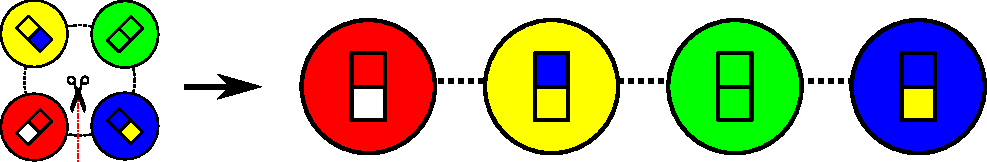
\includegraphics[width=\linewidth]{img/baseball_ligne.pdf}
\end{center}

Puis, \textit{apprenons de nos réussites}. Dans le problème du crêpier, on a résolu le problème en réduisant progressivement sa taille : on place la première crêpe, puis la deuxième etc. On s'est fixé des objectifs intermédiaires qui décomposent le problème en étapes plus simples.

À partir de ces enseignements, on peut construire l'algorithme suivant :

% FIXME formulation complêtement merdique ! un ordi ne pourra pas comprendre ça ...
\begin{itemize}
  \item On coupe le cercle de sorte que la base avec la place vide soit à l'extrémité droite.
  \item On s'occupe des bases les unes après les autres, de gauche à droite.
  \item Pour rapprocher un joueur de sa base, on déplace les joueurs des autres couleurs pour amener le trou à gauche du joueur à déplacer.
  \item On répète l'opération jusqu'à ce que les deux joueurs soient revenus à leur base, et on n'y touche plus.
\end{itemize}

% FIXME tikz ? l'illustration est fausse, la base rouge devrait être à droite.
\begin{center}
  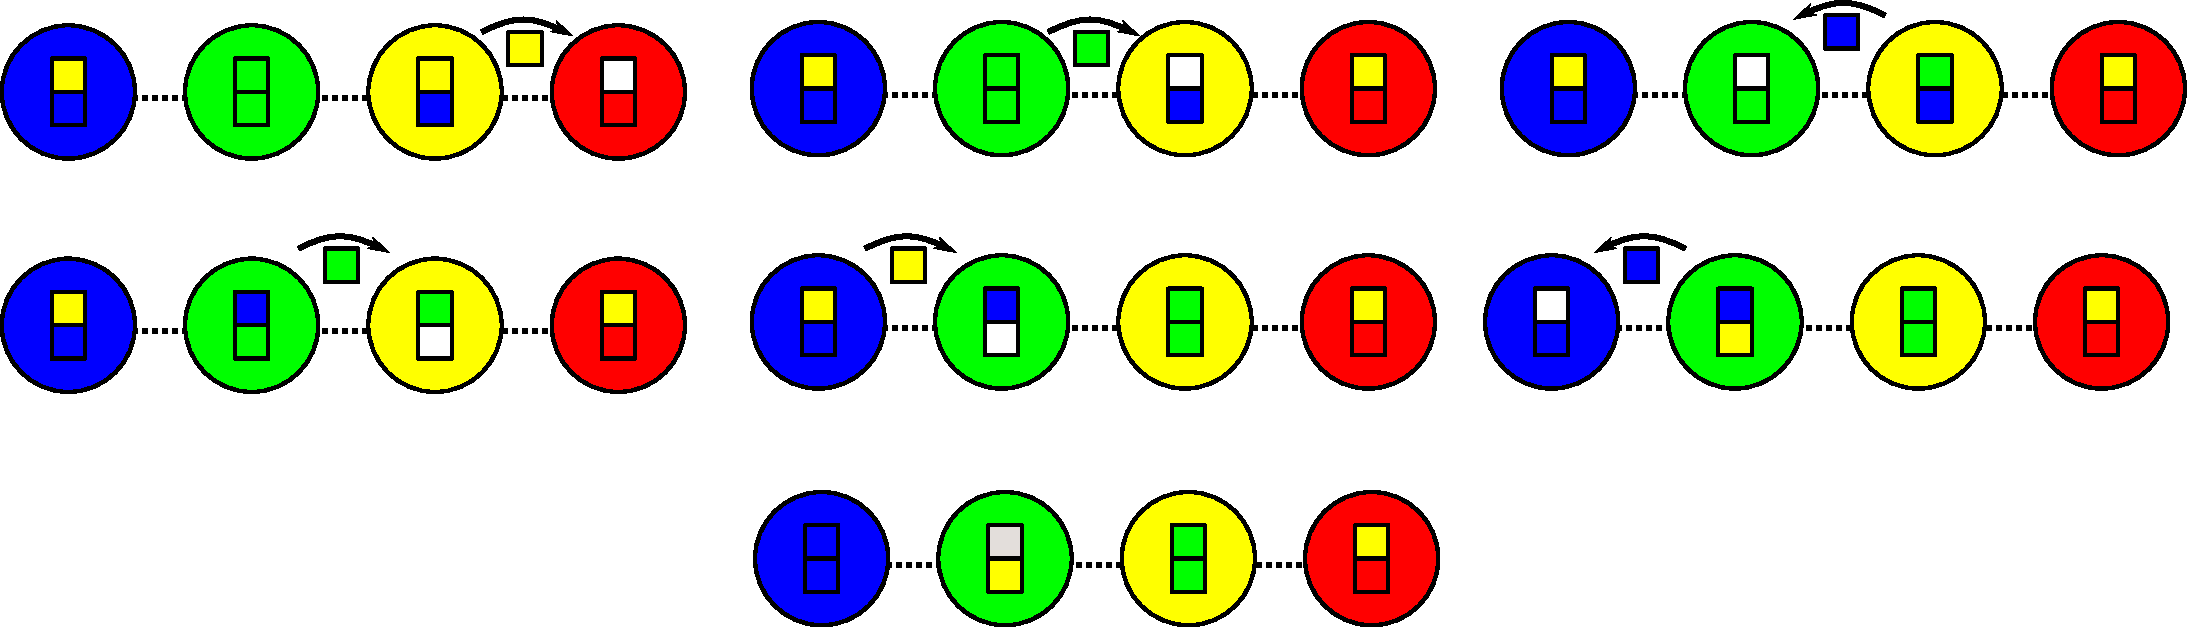
\includegraphics[width=\linewidth]{img/baseball_ex3.pdf}
\end{center}

On peut maintenant ignorer la première base, qui est déjà rentrée.

\section*{Correction d'algorithmes}

Notre deuxième algorithme est un peu plus complexe que le précédent, mais il est correct - une propriété très importante quand on écrit un algorithme. Mais comment être sûr de la \textbf{correction} d'un algorithme ? Il existe plusieurs approches :

\begin{description}
  \item[Tester tous les cas] On vérifie que l'algorithme trouve la solution pour tous les cas possibles. Mais ça ne marche que pour un problème de taille finie, et montrer de cette manière que notre algorithme est correct pour 4 bases n'implique pas sa correction pour 5 bases.
  \item[Écrire une preuve mathématique] On peut prouver mathématiquement que cet algorithme fonctionne pour le cas général $m$ bases. Ce n'est pas trivial, mais les chercheurs en informatique en ont écrite des plus difficiles.
  \item[Ça ressemble à un algo classique] On peut observer une certaine ressemblance avec un algorithme déjà connu. Mais ça ne prouve rien, au fond ...
\end{description}

\subsection*{Les algorithmes classiques}

Les informaticiens apprennent par c\oe{}ur des algorithmes (abstraits) à l'école. Face à un problème nouveau, un informaticien cherche généralement à le ramener à un problème connu. Ce rapprochement se fait en trouvant des analogies ou en décomposant le problème en plusieurs sous-problèmes connus.

Par exemple, quand des collègues informaticiens jouent au crêpier, ils demandent avant tout si c'est \og une tour de Hanoï \fg, jeu bien connu des informaticiens. Pour le base-ball multicolore, notre algorithme ressemble à un \og tri à bulle \fg, autre algorithme bien connu. Mais cette ressemblance ne suffit pas à prouver la correction de notre algorithme. Pour la prouver, il faudrait démontrer que notre algorithme est un cas particulier du tri à bulle.
 
\subsection*{Les algorithmes de tri}

Les algorithmes de tri sont très classiques en informatique. D'une part, ils permettent d'expliquer les grands principes aux élèves («diviser pour régner», récursivité, algorithmes gloutons \ldots). D'autre part, les ordinateurs trient très souvent des données, car beaucoup de problèmes sont plus simples après (trouver un livre est plus simple dans une bibliothèque rangée, par exemple). \textit{Les musiciens font leurs gammes, les informaticiens débutants apprennent leurs algorithmes}

%\subsection*{Le travail des chercheurs}

%Une partie du travail des chercheurs en informatique est d'améliorer les algorithmes connus, d'en inventer de nouveaux et de démontrer leur correction, d'en comparer les performances ...

\chapter*{Le plus court chemin}

Soit un ensemble de villes représenté par des clous plantés dans une planche de bois. Le but du jeu est de trouver le plus court chemin passant une fois et une seule par chaque ville et terminant sur la ville de départ. Pour représenter le chemin, on attache une ficelle à un clou et on la fait passer de clou en clou.

\begin{center}
  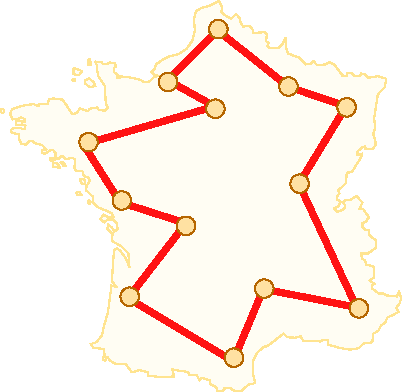
\includegraphics[width=0.5\linewidth]{img/tsp.pdf}
  \label{img:tsp}
\end{center}

\encart{Matériel}{
  \begin{itemize}
  \item Une planche avec des trous au hasard,
  \item autant de longs clous que de trous,
  \item une ficelle suffisamment longue et \textbf{qui ne soit pas élastique},
  \item un marqueur.
  \end{itemize}
}

Il existe un grand nombre de chemins possibles. Arriverez vous à trouver le plus court ?

\newpage

\section*{Recherche de la solution optimale}

Ce problème a de nombreuses applications dans la vie de tous les jours : minimiser la tournée du facteur, la longueur des pistes d'un circuit imprimé, les déplacements d'un bras robotique \ldots C'est un problème très étudié, plus connu sous le nom de \textbf{\og problème du voyageur de commerce \fg}.

Le problème du voyageur de commerce appartient à une catégorie de problèmes très difficiles à résoudre. Pour ces problèmes, on ne dispose pas d'algorithmes assez performants pour le résoudre quand $n$ est élevé. Le problème du voyageur de commerce ayant fait l'objet de nombreuses études, beaucoup d'algorithmes ont été proposés pour le résoudre le plus efficacement possible.

\subsection*{Comparaison de deux algorithmes}

L'approche naïve consiste à calculer la longueur de tous les chemins possibles, et comparer les résultats pour ne retenir que le plus court. Pour $n$ villes, le nombre de chemins possible est $n!$. La performance de l'algorithme est donc $O(n!)$.

Il existe cependant des algorithmes plus efficaces - par exemple, l'algorithme de Held-Karp a une performance de $O(n^{2}2^n)$. Pour illustrer la différence, comparons l'augmentation des calculs nécessaires à mesure que $n$ augmente :

\begin{center}
  \begin{tabular}{|l|llll|}
    \hline
    nombre de sommets       & $5$   & $10$      & $15$            & $20$ \\
    \hline
    %méthode naïve $O(n!)$   & 120 & 3628800 & 1307674368000 & 2432902008176640000 \\
    %Held-Karp $O(n^{2}2^n)$ & 800 & 102400  & 7372800       & 419430400 \\
    méthode naïve $O(n!)$   & $120$ & $3628800$ & $1.3 \times 10^{12}$ & $2.4 \times 10^{18}$ \\
    Held-Karp $O(n^{2}2^n)$ & $800$ & $102400$  & $7.3 \times 10^6$       & $4.1 \times 10^8$ \\
    \hline
  \end{tabular} 
\end{center}

Ce tableau indique qu'en testant un milliard de chemins par seconde, il faudrait à la méthode naïve plus de \textbf{77 ans} pour trouver le chemin le plus court entre 20 sommets ! Dans les mêmes conditions, l'algorithme Held-Karp met moins d'\textbf{une demi-seconde} pour trouver le même résultat.

  \begin{center}
    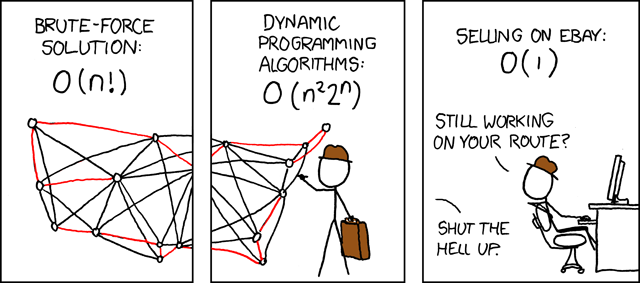
\includegraphics[width=\linewidth]{img/tsp_xkcd.png}
    \label{img:tsp_xkcd}
  \end{center}

\section*{Recherche d'une solution approchée}

Pour ces problèmes complexes, on préfère souvent trouver une solution raisonnablement bonne (solution approchée) très rapidement, plutôt que de chercher très longtemps la solution optimale. Une \textbf{heuristique} est une méthode pour fouiller intelligemment l'espace des solutions possibles à la recherche des bonnes solutions. La recherche d'heuristiques efficaces fait parti du travail des chercheurs en informatique.

\subsection*{Heuristique : le plus proche voisin}

Partez d'une ville, et allez vers la ville la plus proche par laquelle vous n'êtes pas encore passé. Recommencez, jusqu'à passer par toutes les villes, et revenez au point de départ. Cette heuristique aura tendance à prendre de préférence les distances les plus courtes ... Mais elle n'aboutira pas forcément la meilleure solution. Par exemple :

\begin{center}
  \begin{tikzpicture}[scale=0.45,point/.style={shape=circle,draw}]

%\draw [step=1,thin,color=gray] (-16,-3) grid (9,3);

\node [point] 	(A) at (0,0) {A};
\node [point] 	(B) at (2,0) {B};
\node [point] 	(C) at (-3,0) {C};
\node [point] 	(D) at (8,0) {D};
\node [point] 	(E) at (-15,0) {E};

\draw [thick,->] (A) to [bend left=30] (B);
\draw [thick,->] (B) to [bend left=30] (C);
\draw [thick,->] (C) to [bend left=30] (D);
\draw [thick,->] (D) to [bend left=20] (E);
\draw [thick,->,dashed] (E) to [bend left=30] (A);

\draw [thick,->,color=red] (E) to (C);
\draw [thick,->,color=red] (C) to (A);
\draw [thick,->,color=red] (A) to (B);
\draw [thick,->,color=red] (B) to (D);
\draw [thick,->,color=red,dashed] (D) to [bend left=15] (E);

\end{tikzpicture}

\end{center}

Si on démarre de \tikz \node [shape=circle,draw] {A};, aller toujours vers le voisin le plus proche nous fait faire un trajet (\tikz \draw[->](0,0) -- (0.5,0);) beaucoup plus long que le trajet optimal (\tikz \draw [->,color=red] (0,0) -- (0.5,0);).

\subsection*{Heuristiques et méta-heuristiques}

Une heuristique est spécifique au problème qu'elle traite : elle exploite certaines propriétés du problème pour orienter la recherche vers des \og régions \fg susceptibles de contenir des bonnes solutions. Cependant, certaines heuristiques reposent sur des concepts assez génériques pour s'appliquer à de nombreux problèmes, moyennant quelques adaptations. On parle alors de \textbf{méta-heuristiques}. Les méta-heuristiques sont souvent inspirées de la nature. En voici quelques exemples.

\begin{description}
  \item[Le recuit-simulé] s'inspire d'un processus utilisé en métallurgie pour minimiser l'énergie d'un matériau.
  \item[Les colonies de fourmis] s'inspirent du comportement des insectes sociaux : avez vous remarqué que les fourmis finissent toujours par trouver le chemin le plus court entre la fourmilière et la source de nourriture ?
  \item[Les algorithmes génétiques] reproduisent les mécanismes de l'évolution dans le vivant :
    \begin{itemize}
      \item une population de solutions aléatoires est créée ;
      \item on soumet cette population à une sélection naturelle (les meilleures solutions sont les plus adaptées) ;
      \item on créé de nouvelles solutions à partir des solutions existantes par croisements et mutations ;
    \end{itemize}
    Génération après génération, on observe une amélioration des solutions.
\end{description}


\chapter*{Le coin de l'animateur}
\label{chap:coin-animateur}

Pour que le déroulement des activités se passe bien, voici quelques conseils.

\encart{Remarques générales}{
  \begin{itemize}
  \item Appropriez vous les activités. Pratiquez-les à l'avance et n'hésitez pas à ne pas suivre les consignes à la lettre.
  \item Ces activités sont des bases de discussion avec les participants, il n'y a pas d'évaluation à la fin.
  \item Evitez les introductions théoriques ; commencez par les activités, elles serviront de support pour discuter de la théorie.
  \end{itemize}
}

\section*{Le jeu de Nim}

L'objectif de cette activité est simplement d'introduire la notion d'algorithme comme stratégie gagnante pour un problème donné.

\begin{itemize}
  \item Commencez par jouer avec les participants, sans dire qu'il y a un truc. Si vous jouez bien, vous gagnerez à tous les coups.
  \item Bien sûr, pour gagner, vous devez laisser votre adversaire commencer. S'il insiste pour ne pas commencer, vous pouvez toujours essayer de gagner en ratrappant la stratégie gagnante à la première erreur.
  \item Si un participant connaît déjà la stratégie gagnante du jeu, il pourra vous remplacer pour jouer avec les autres participants.
  \item Si vous n'êtes pas sûr d'appliquer correctement la stratégie gagnante, proposez un match en 3 - ou en 5, en cas de coup dur ;)
  \item Pour amener les participants à découvrir la stratégie gagnante, vous pouvez grouper les objets par 4, rendant ainsi l'astuce plus visible.
\end{itemize}

\section*{Le crêpier psycho-rigide}

L'objectif de cette activité est de trouver un algorithme, de le faire verbaliser par les participants et d'en mesurer la performance.

\begin{itemize}
  \item Expliquez les règles et demandez aux participants de tenter de résoudre le problème ;
  \item s'ils bloquent, conseillez-les. Par exemple : \og essaye d'abord de mettre la grande crêpe en bas \fg, ou encore \og où doit se trouver la grande crêpe pour pouvoir l'amener en bas ? \fg
  \item Quand les participants ont trouvé l'algorithme, demandez leur de l'expliquer. 
  \item Demandez ensuite de calculer le nombre de coups nécessaires pour ranger la pile de crêpes. Le nombre de coups dépendant de l'état initial, faites les généraliser en trouvant le nombre de coups maximal pour ranger une crêpe, puis $n$ crêpes.
\end{itemize}

\section*{Le base-ball multicolore}

L'objectif de cette activité est d'introduire la notion de correction d'algorithme.

\begin{itemize}
  \item Il faut laisser les participants chercher un peu en les faisant verbaliser
  \item S'ils sont sur le point de trouver l'algo juste, on introduit très vite l'algo faux pour préserver un enchaînement logique: ``oui, ok, mais je vais vous montrer une façon de faire rigolote''
  \item Quand l'algo juste est établi, et avant de parler de performance, on peut partir sur une variante :
    \begin{itemize}
    \item Chaque participant prend une couleur (une base placée au sol entre ses pieds)
    \item Chaque participant (sauf 1) prend un bonhomme dans chaque main
    \item À chaque étape, celui qui a une main libre prend un bonhomme dans la main d'un voisin
    \item (attention, c'est fastidieux à 8 ou 9 couleurs, il vaut mieux faire deux rondes car l'algo semble $O(n^2)$)
    \end{itemize}
  \item Expérimentalement, l'algo qui tourne converge très souvent vers la solution à 5 bases, mais converge souvent vers la boucle infinie quand il y a plus de couleurs. Ne tentez pas le diable ;)
  \item Dans la disposition linéaire, il est plus simple de mettre la couleur avec un seul bonhomme à une extrémité, et commencer par remplir la maison de l'autre extrémité. Sinon, on se retrouve avec une maison remplie de un seul au milieu, et il faut comprendre que la solution passe par le stockage temporaire d'un pion de la maison d'à coté sur le trou.
  \item Le discours sur le $O(n)$ est volontairement approximatif. On veut faire sentir les choses; faire un vrai cours prend une douzaine d'heures (cf. \url{http://www.loria.fr/~quinson/Teaching/TOP/}).
  \item Il serait intéressant de prouver effectivement la correction de l'algorithme linéaire, ainsi que de quantifier la probabilité de fonctionnement de l'algo qui tourne en fonction du nombre de maisons
  \item Au passage, le crépier ne ressemble pas du tout aux tours de Hanoï: l'histoire ressemble un peu, mais la résolution est très différente (il y a $2^n-1$ étapes à Hanoï et $3\times n$ au crépier\ldots)
\end{itemize}

\section*{Le plus court chemin}

L'objectif de cette activité est d'introduire la notion de complexité des problèmes.

\begin{itemize}
  \item Commencez par donner un exemple de chemin, en faisant volontairement des détours. Laissez ensuite les participants trouver de meilleures solutions. 
  \item À mesure qu'ils avancent, il sera de plus en plus difficile d'améliorer les résultats. Insistez sur le fait que lorsqu'ils trouvent une meilleure solution, ils ne peuvent pas être sûr qu'il n'en existe pas une meilleure.
  \item Pour qu'ils se fassent une idée de la complexité du problème, vous pouvez demander aux participants de calculer le nombre de chemins possibles ($n!$), et les amener à refaire l'estimation du temps de calcul nécessaire à raison d'un milliard de chemins testés par seconde.
\end{itemize}

\end{document}
